\section{Quelques définitions}
Informatique
Algorithmique
Programmation

\section{Architecture matérielle d'un ordinateur}
\subsection{Modèle de Von Neumann}

 ouvoir exécuter des algorithmes arbitraires, les ordinateurs actuels sont tous bâtis
autour du même modèle architectural théorique, l’architecture de Von Neumann, même
si la mise en œuvre pratique est un peu plus complexe.

Le premier ordinateur électronique fut l’ENIAC
(dont le but était de calculer des tables indiquant les paramètres de tir d’une batterie d’artillerie
en fonction de la distance de l’objectif, du vent, etc.) dont la construction démarra
en 1943. 
Son architecture a été décrite dans un rapport de John Von Neumann en 1945 et
est depuis appelée «~architecture de Von Neumann~». Depuis près de 70 ans, à quelques variations
près, cette  architecture sert de base à la plupart des systèmes à microprocesseur actuel. 
%\begin{figure}[h]

\begin{minipage}[c]{.49\linewidth}
Elle est composée des éléments suivants :
\begin{itemize}
\item d'une mémoire vive ;
\item d'un processeur qu'on peut conceptuellement décomposer en une unité de contrôle et
une unité de calcul arithmétique et logique ;
\item de dispositifs périphériques, appelés simplement périphériques ;
\item d'un canal de communication entre la mémoire, le processeur et les périphériques, appelé
le bus.
\end{itemize}
\end{minipage} \hfill
\begin{minipage}[c]{.49\linewidth}
\begin{center}
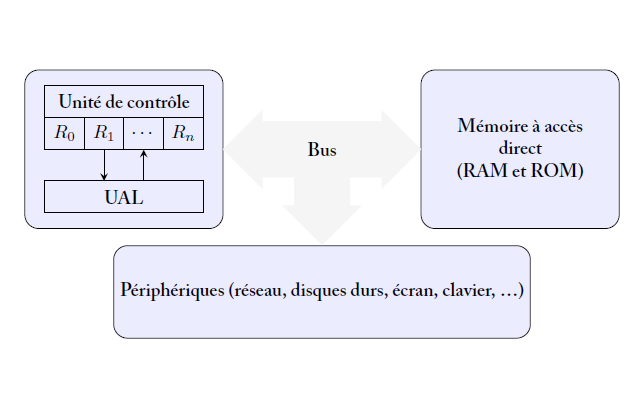
\includegraphics[width=.99\textwidth]{von.png}
%\caption{Architecture de Von Neumann}
%\label{}
\end{center}
\end{minipage}
%\end{figure}

\subsection{La carte mère et ses composants}
\subsubsection{La carte mère}
\noindent
\begin{minipage}[c]{.49\linewidth}
\noindent La carte mère est un des éléments central de l'ordinateur. Elle assure la liaison avec le boîtier, mais surtout, elle comporte : 
\begin{itemize}
\item l'interface avec le processeur \textit{via} le socket (le socket de la carte mère est à choisir en fonction du processeur souhaité);
\item les connecteurs permettant de brancher la mémoire RAM;
\item le BIOS;
\item les connecteurs SATA permettant par exemple de relier le disque dur;
\item la carte son et souvent la carte graphique;
\item les connecteurs USB, audio, video (VGA ou HDMI), RJ45... permettant la connexion des différents périphériques;
\item des ports PCI (PCI-Express) permettant de connecter des cartes d'interfaces supplémentaires \textit{etc}.
\end{itemize}
\end{minipage} \hfill
\begin{minipage}[c]{.49\linewidth}
\begin{center}
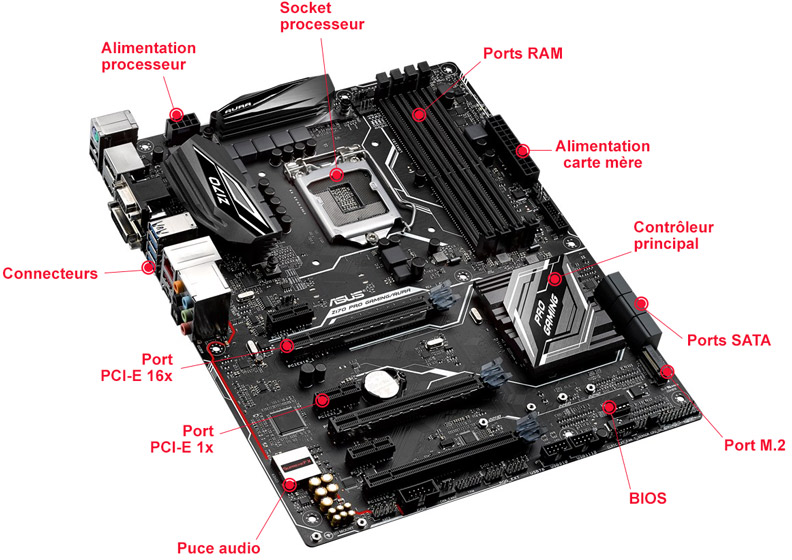
\includegraphics[width=\linewidth]{fig_01_CarteMere}
\end{center}
\end{minipage}

\subsubsection{Le processeur}
\begin{minipage}[c]{.65\linewidth}
Le processeur (ou unité centrale de traitement) est le composant exécutant toutes les opérations de base. La fréquence d'un processeur, s'exprime en Ghz. Il s'agit du nombre d'opérations qu'il peut faire par seconde.

En effet, un processeur peut-être multi-c\oe{}ur, c'est-à-dire qu'il possède plusieurs c\oe{}urs physiques fonctionnant de façon simultanée. Un processeur multi-c\oe{}ur permet de réaliser des opérations simultanées (à condition que le système d'exploitation puisse le gérer). 
De plus, il existe des processeurs multi-thread permettant d'exécuter plusieurs tâches en parallèles (sur le même processeur). 

En conséquence, pour comparer la rapidité de deux processeurs, la fréquence ne suffit pas, le nombre de cœurs et le nombre de threads sont à prendre en compte. 

\end{minipage}\hfill
\begin{minipage}[c]{.3\linewidth}
\begin{center}
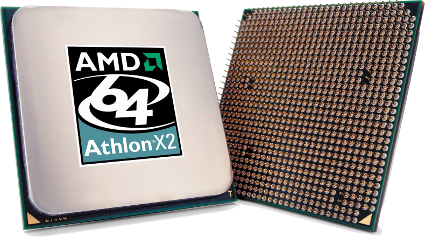
\includegraphics[width=.8\textwidth]{cpu_amd_p.png}
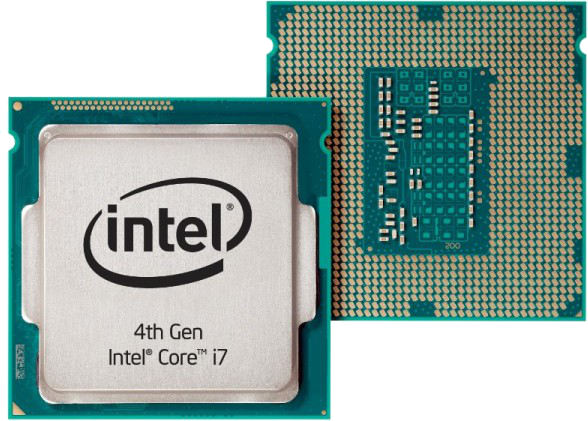
\includegraphics[width=.8\textwidth]{cpu_intel.png}
\end{center}
\end{minipage}
\subsubsection{Notion de bus}
En informatique, le terme bus désigne un ensemble de fils support de l'information et organe de communication entre différents composants.Il existe deux grands types de bus :
\begin{itemize}
\item le bus série : il comporte plusieurs fils, dont la masse (référence de potentiel), le fil de données, le fil d'horloge. Les données sont transmises en série;
\item le bus parallèle : il comporte un fil de masse, un fil d'horloge, et $n$ fils de données pour un bus $n$ bits ; les données sont transmises en parallèle.  
\end{itemize}

Par ailleurs, des bus sont intégrés dans des puces. Par exemple, dans les microprocesseurs, les différents constituants communiquent entre eux par des bus parallèles. Ainsi, sur la carte mère, la communication est assurée par :
\begin{itemize}
\item le bus système qui relie le micorprocesseur au chipset;
\item le bus mémoire qui relie le chipset à la mémoire vive;
\item le bus d'extension qui relie le chipset aux connecteurs d'entrée -- sortie.
\end{itemize}

	
Sur la carte mère sont intégrés différents bus parallèles que l'on peut même parfois distinguer. Ces bus permettent de relier les différents constituants entre eux afin qu'ils communiquent. On retrouve des bus d'adresses, de données et de contrôle.

Entre la carte mère et les différents périphériques (disque dur par exemple), on utilise de plus en plus des bus séries. Ainsi, après le tout IDE, bus parallèle qui a été massivement utilisé dans les ordinateurs grand public, le bus SATA est de plus en plus utilisé. 
\vspace{.25cm}


\noindent \begin{minipage}[c]{.7\linewidth}
Plusieurs normes SATA ont été développées. 
Cette technologie présente des débits bien plus importants que les disques durs mécaniques  (60 Mo/s au mieux) mais s'adapte bien aux débits des SSD qui avoisinent les \SI{500}{Mo/s}.
\end{minipage} \hfill
\begin{minipage}[c]{.29\linewidth}
\begin{center}
\begin{tabular}{|c|c|}
\hline
Norme & Débit (Mo/s) \\
\hline
SATA I & 187,5 \\ \hline
SATA II & 375 \\ \hline
SATA III & 750 \\ \hline
\end{tabular}
\end{center}
\end{minipage}



\subsection{Les mémoires}
\subsubsection{Les mémoires de masse -- Disque dur}

\begin{minipage}[c]{.6\linewidth}
Un disque dur (non SSD) est composé de disques rigides et paramagnétiques (en aluminium, en verre ou en céramique) recouverts d'une couche magnétique et d'un film protecteur. Ces plateaux sont entraînés par un moteur électrique dont la fréquence de rotation est fixe. La fréquence de rotation peut atteindre les \SI{15 000}{tr.min^{-1}}. Un bras, sur lequel sont fixées les têtes de lecture -- écriture, est aussi motorisé pour atteindre les différentes parties du disque. La distance entre les têtes et les plateaux est de l'ordre de 10 \textit{nm}. Elle est maintenue par un coussin d'air formé par la rotation des disques. 
\end{minipage} \hfill
\begin{minipage}[c]{.35\linewidth}
\begin{center}
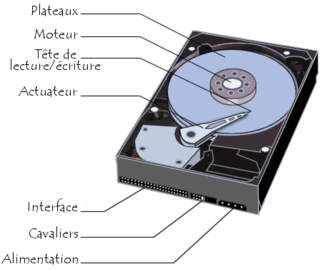
\includegraphics[width=.9\textwidth]{dd_comp.png}
\end{center}
\end{minipage} 

Les têtes de lecture -- écriture sont inductives et permettent de générer un champ magnétique dans deux sens opposés permettant de polariser la couche magnétique du disque. Ainsi, en mode lecture les changements de polarité sont transcrits par un convertisseur analogique numérique (CAN) en bits (0 ou 1).

Les données sont organisées en pistes concentriques, les données les plus rapidement accessibles étant celles situées sur le disque extérieur. Chaque piste est divisée en secteurs (d'un minimum de 512 octets). Enfin, on appelle cylindre l'ensemble de données situé sur une même piste mais sur un plateau différent. 


La capacité des disques durs atteint les 4 To (téraoctet). Lorsqu'ils sont connectés en SATA, le débit oscille entre 30 et 60 \textit{Mo/s} et peut atteindre les 600 \textit{Mo/s}. Enfin, pour améliorer les performances d'accès aux données, ils possèdent une mémoire cache pouvant aller jusqu'à 128 \textit{Mo} sur laquelle sont stockées les informations fréquemment utilisées. 

Les performances des disques SSD (\textit{Solid State Drive}) sont supérieures à celles des disques durs classiques. Deux critères penchent néanmoins en sa défaveur. D'une part le prix du Go est presque 10 fois plus élevé 
que pour un disque dur mécanique. D'autre part, certaines technologies de SSD présentent l'inconvénient d'être limité en nombre de cycles d'écriture -- lecture.


\begin{center}
\begin{tabular}{|l|l|l|}
\hline
\textbf{Caractéristiques} & \textbf{Disque dur mécanique} & \textbf{SSD} \\ \hline
Temps d'accès & En moyenne 12ms & 0.1ms \\ \hline
Poids & De 400g à 700g & Quelques dizaines de grammes \\ \hline
Consommation en veille & De l'ordre du Watt & 100 mW \\ \hline
Consommation en activité & 4W environ & 900 mW \\ \hline
Bruit  & En moyenne 40 dB & 0 dB\\ \hline
\end{tabular}
\end{center}


\subsubsection{La mémoire cache et mémoire vive (RAM)}
La mémoire cache est une mémoire très rapide que l'on trouve par exemple sur les microprocesseurs ou sur les disques durs. Dans le cas des microprocesseurs, elle est située au plus proche de ceux-ci et permet d'accélérer l'exécution des programmes. 

La mémoire vive (RAM) est plus rapide d'accès qu'un disque dur (de 1000 à 10\, 000 dois plus rapide), mais plus lente qu'une mémoire cache.  Elle permet de stocker (à court terme) des données. C'est elle qui permet d'utiliser plusieurs applications en même temps et de passer rapidement de l'une à l'autre. 



\subsection{Communication avec les périphériques}
\subsubsection{Le port USB \cite{usb}}

\noindent \begin{minipage}[c]{.75\linewidth}
USB (\textit{Universal Serial Bus} -- bus série universel) est un protocole de communication apparu en 1996 (USB 1.0). Ce protocole série a révolutionné les connexions entre PC et périphériques en instaurant un environnement « tout USB », uniformisant les modes de communication avec l'ordinateur... C'est sans doute le bus de communication le plus utilisé. Ses principaux concurrents sont désormais les protocoles sans fil Bluetooth et WiFi.
\end{minipage}\hfill
\begin{minipage}[c]{.2\linewidth}
\begin{center}
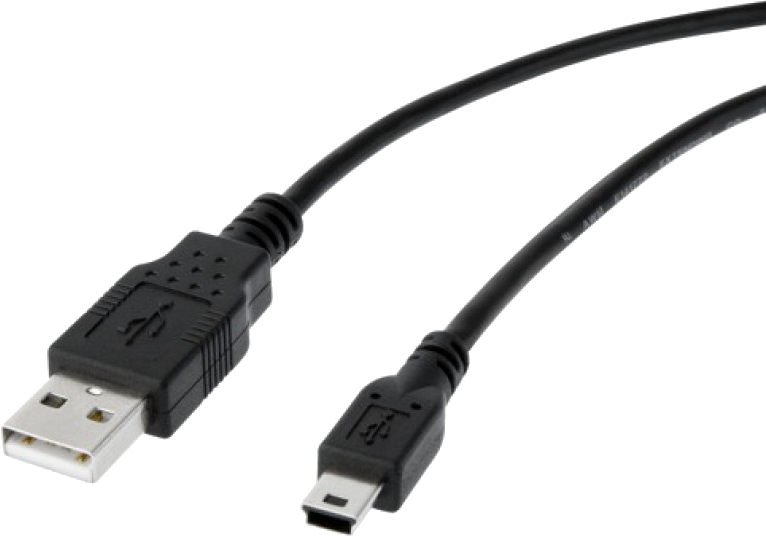
\includegraphics[width=\textwidth]{usb.png}
\end{center}
\end{minipage}

\begin{center}
\begin{tabular}{|l|l|l|l|l|}
\hline
Version & USB 1.0 & USB 1.1 & USB 2.0 & USB 3.0 \\ \hline
Débit   & \SI{0,19}{Mo.s^{-1}} & \SI{1,5}{Mo.s^{-1}} & \SI{60}{Mo.s^{-1}} & \SI{600}{Mo.s^{-1}}  \\ \hline
\end{tabular}
\end{center}

Un connecteur USB est composé de 4 fils : 
\begin{itemize}
\item un fil d'alimentation (5V -- VBUS);
\item un fil de masse (GND);
\item deux fils de données (D+ et D- torsadés). 
\end{itemize}

Afin de faire transiter l'information, l'USB utilise des paquets. Ainsi une transaction USB est composée de 3 paquets :
\begin{itemize}
\item le paquet \textit{token} contient des informations sur la nature de la communication (est-ce l'hôte ou le périphérique qui envoie de l'information ?);
\item le paquet de données;
\item le paquet \textit{handshake} qui contient des informations sur le déroulement de la transaction (le paquet a été reçu correctement, interruptions lors de la transaction...).
\end{itemize}


\subsubsection{Le port série}

Pour les communications séries, les connecteurs sont de type D-SUB (DB9 par exemple).

Historiquement, le port série est le premier port de communication utilisant une transmission série (norme RS232). Son débit est au maximum de 19200 bps (bits par seconde). Il a été très longtemps utilisé pour sa simplicité de configuration et de pilotage. C'est d'ailleurs le protocole de communication mis en œuvre pour un grand nombre de système du laboratoire : MAXPID, cordeuse, DAE, etc. A noter cependant que si certains PC ont encore un port COM1 RS232, la plupart utilise un adaptateur RS232-USB pour communiquer avec le PC.

\subsubsection{Le port parallèle}
Pour les communications séries, les connecteurs sont de type D-SUB (DB25 par exemple).

Le port parallèle est un port reposant sur un protocole unidirectionnel de communication parallèle. Il est en voie d'extinction, comme le port série RS232. Il était le plus souvent utilisé pour la communication PC--imprimante. Le débit maximum  est de 16Mbps.


\subsubsection{Port PS/2 -- \textit{Personal System/2}}

\begin{minipage}[c]{.75\linewidth}
Le port PS/2 utilise un connecteur mini-din. 
Ce port de communication de taille réduite a succédé au PS/1 (Din, le même en plus encombrant ) permettant la connexion du clavier et/ou de la souris créé par IBM (1987) mais démocratisé en 1995 suite à son intégration sur les cartes mères type ATX. 

Il est également supplanté par le standard USB depuis quelques années mais également de plus en plus par le bluetooth.
\end{minipage}\hfill
\begin{minipage}[c]{.2\linewidth}
\begin{center}
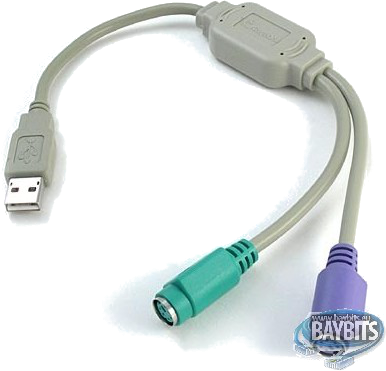
\includegraphics[width=\textwidth]{ps2.png}
\end{center}
\end{minipage}


\subsection{Communication réseau}
\subsubsection{Port RJ45 -- \textit{Registered Jack}}

\begin{minipage}[c]{.7\linewidth}
Ce port permet la connexion filaire réseau ethernet (LAN : Local Area Network) par câble. Différents protocoles existent, spécifiant différents débits.

\begin{center}
\begin{tabular}{|c|c|c|c|}
\hline
Protocole & Gigabits & 10GBase-X & 100GBase-X \\ \hline
Débit & 128 Mo/s & 1280 Mo/s & 12 800 Mo/s\\ \hline
\end{tabular}
\end{center}


\end{minipage}\hfill
\begin{minipage}[c]{.25\linewidth}
\begin{center}
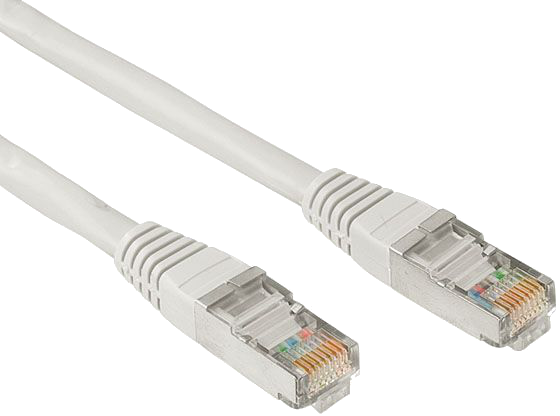
\includegraphics[width=.9\textwidth]{ethernet.png}
\end{center}
\end{minipage}\hfill



\subsubsection{Wi-Fi}

Le Wi-Fi (\textit{Wireless Fidelity} -- Norme \textit{IEEE 802.11}) est un standard définissant les caractéristiques d'un réseau local sans fil. La liaison est assurée par l'intermédiaire d'ondes électromagnétiques.  

Différentes normes physiques définissent le débit de la transmission en fonction de la portée. 
\begin{center}
\begin{tabular}{|c|c|c|c|}
\hline
\textbf{Standard} & \textbf{Bande de fréquence} & \textbf{Débit} & \textbf{Portée} \\ \hline
WiFi a (802.11a) & 5 GHz & 54 Mbit/s & 10 m \\ \hline
WiFi B (802.11b) & 2,4 GHz -- 2,5 GHz& 11 Mbit/s & 100 m \\ \hline
WiFi G (802.11g) & 2,4 GHz -- 2,5 GHz & 54 Mbit/s & 75 m \\ \hline
WiFi N (802.11n) & 2,4 GHz ou 5 & 450 Mbit/s & 125 m \\ \hline
\end{tabular}
\end{center}


\subsubsection{3G -- 4G}
La 3G et la 4G sont les troisième et les quatrième générations de transmissions de données pour la téléphonie mobile. La 4G permet d'avoir accès à des débits théoriques très supérieurs à la 3G et possède un c\oe{}ur de réseau basé sur IP. 

\textit{Tableau récapitulatif \url{http://www.commentcamarche.net/}}
\begin{center}
\begin{tabular}{|c|c|p{6cm}|c|c|}
\hline
Standard	& Génération	&Bande de fréquence	& Débit & \\
\hline 
GSM	& 2G & Permet le transfert de voix ou de données numériques de faible volume.&	9,6 kpbs	&9,6  kpbs \\ \hline
GPRS &2.5G & Permet le transfert de voix ou de données numériques de volume modéré.&	21,4-171,2 kpbs	&48 kpbs \\ \hline
EDGE & 2.75G & 	Permet le transfert simultanés de voix et de données numériques.&	43,2-345,6 kbps&	171 kbps \\ \hline
UMTS & 3G &Permet le transfert simultanés de voix et de données numériques à haut débit.&	0.144-2 Mbps	&384 Kbps \\ \hline
LTE & 4G	& Permet le transfert simultanés de voix et de données numériques à haut débit.&	10-300 Mbps	&5-75 Mbps \\ \hline
\end{tabular}
\end{center}

\subsection{Son et vidéo}




\begin{minipage}[c]{.85\linewidth}
Le port VGA -- \textit{Video Graphics Array}

Le connecteur est de type D-SUB, ici DE-15. Ce port est de type analogique.

\end{minipage} \hfill
\begin{minipage}[c]{.14\linewidth}
\begin{center}
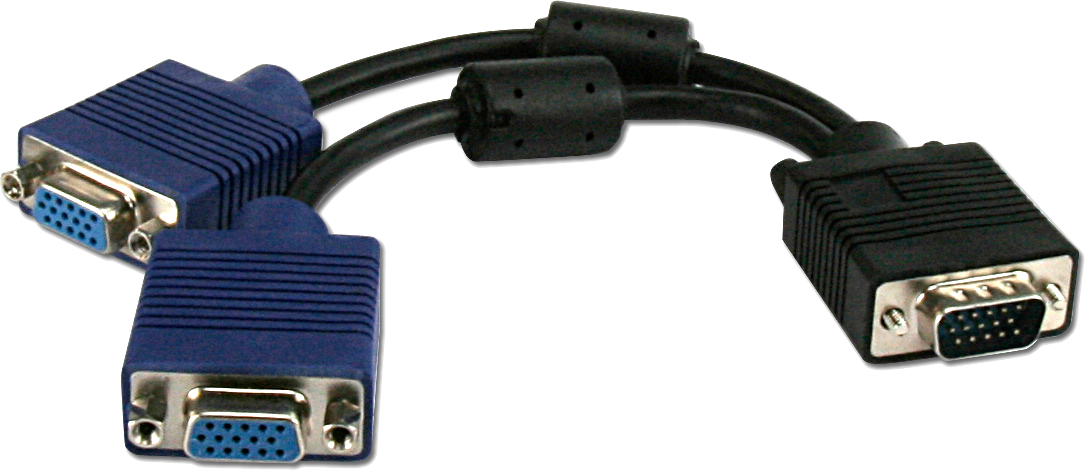
\includegraphics[width=.9\linewidth]{vga}
\end{center}
\end{minipage}


\begin{minipage}[c]{.85\linewidth}
Le port DVI -- \textit{Digital Visual Interface}

Ce port est de type numérique non HD. Il apporte une amélioration en terme de réduction du bruit par rapport au connecteur VGA analogique.
\end{minipage} \hfill
\begin{minipage}[c]{.14\linewidth}
\begin{center}
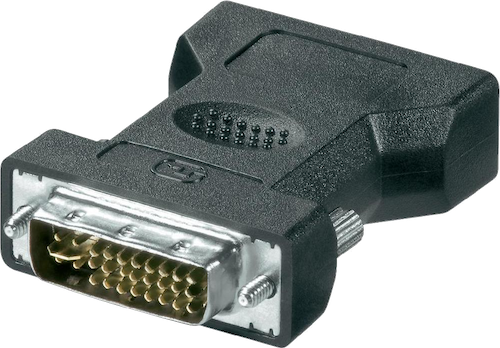
\includegraphics[width=.9\linewidth]{dvi}
\end{center}
\end{minipage}


\begin{minipage}[c]{.85\linewidth}
Le port HDMI -- \textit{High Definition Multimedia Interface}

Il s'agit d'une interface audio vidéo totalement numérique permettant de raccorder un lecteur de disque, une console, un décodeur \textit{etc.} à un écran de télévision haute définition.
\end{minipage} \hfill
\begin{minipage}[c]{.14\linewidth}
\begin{center}
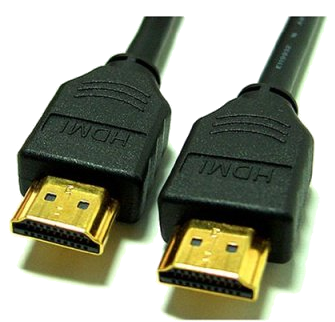
\includegraphics[width=.9\linewidth]{hdmi}
\end{center}
\end{minipage}


\section{Système d'exploitation -- Operating Systems (OS)}
\subsection{Présentation}

Dans le cadre du modèle de la machine de von Neumann, un seul programme s’exécute. Il s'agit donc du système d'exploitation qui est chargé dès le démarrage.  Ce programme a pour but de gérer les accés aux processeurs et à la mémoire et aux périphériques, ce qui permet
effectivement que l’ordinateur exécute plusieurs programmes à la fois.

Par ailleurs l'OS permet de manière générale de gérer l'organisation des données sur le disque dur ainsi que leur droit d'accès. Il gère aussi les différentes ressources et sert de garde-fou en cas de tentative de mauvaise utilisation des ressources de l'ordinateur.

Pour finir, l'OS permet à un ou plusieurs utilisateurs de s'identifier leur permettant ainsi d'utiliser un seul ordinateur sans nécessairement partager les données et les programmes. 



\subsection{Exemples d'OS}
Il existe deux grandes familles d'OS : Windows et UNIX. UNIX est elle-même une grande famille derrière laquelle on peut retrouver beaucoup de distributions:  GNU/Linux (Debian, Ubuntu, \textit{etc.}), FreeBSD, MacOS, \textit{etc}. Les différences pouvant être mises en avant sont les suivantes:
\begin{itemize}
\item sous UNIX, il existe des distributions dont les sources sont libres (modifiable par tous);
\item sous UNIX, l'accès à un shell, permet de réaliser une multitude de tâche en ligne de commande, ce qui est parfois plus efficace qu'avec la souris;
\item sous UNIX, la base de logiciels disponibles est centralisée, ce qui peut faciliter la recherche d'un logiciel et son installation;
\item sous Windows, lest installations de périphériques est souvent plus aisée. 
\end{itemize}

Les distributions UNIX sont beaucoup plus répandues qu'on peut parfois le penser : un grand nombre de calculateurs et de serveurs sont sous UNIX, les smartphones, tablettes, box internet sont sous UNIX.



\begin{minipage}[c]{.3\linewidth}
\begin{center}
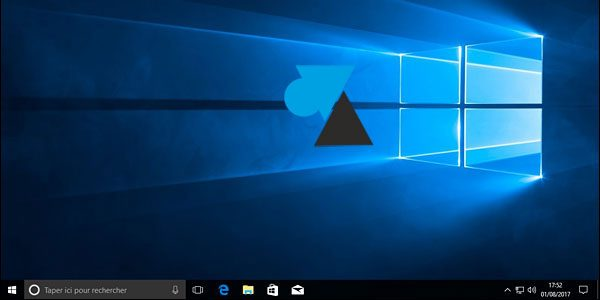
\includegraphics[width=\linewidth]{bureau_win}

\textit{Bureau Windows 10}
\end{center}
\end{minipage} \hfill
\begin{minipage}[c]{.3\linewidth}
\begin{center}
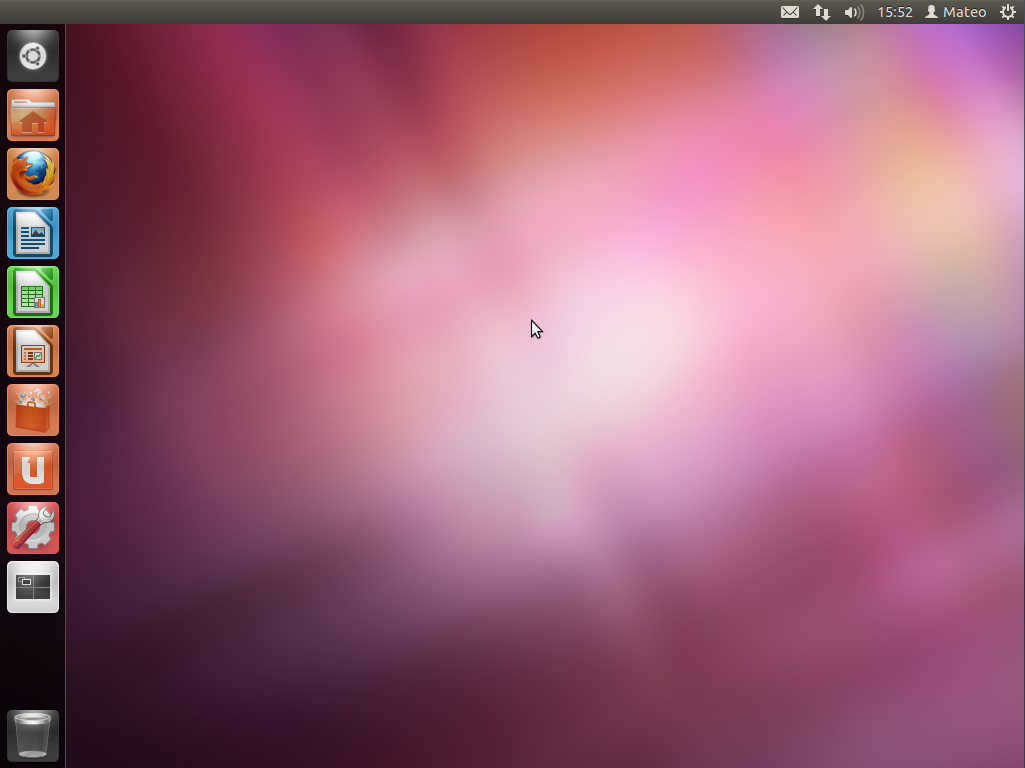
\includegraphics[width=\linewidth]{bureau_ubuntu}

\textit{Bureau Ubuntu}
\end{center}
\end{minipage} \hfill
\begin{minipage}[c]{.3\linewidth}
\begin{center}
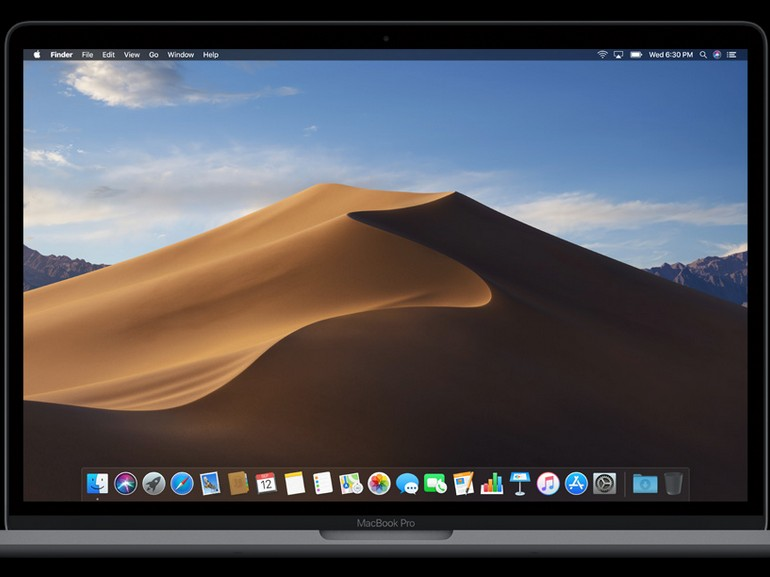
\includegraphics[width=\linewidth]{bureau_mac}

\textit{Bureau MacOS}
\end{center}
\end{minipage} 

\subsection{Organisation des fichiers}
L'organisation des fichiers est totalement différente entre un environnement Windows et un environnement UNIX. 
En première approximation, sous Windows, les fichiers sont triés d'une part par applications. D'autre part, les fichiers utilisateurs sont stockés dans le dossier C:\textbackslash Users.

Sous UNIX, les fichiers sont triés par type de fichiers puis par applications. D'autre part, les fichiers utilisateurs sont stockés dans le dossier \textbackslash home.


\begin{minipage}[c]{.49\linewidth}
\begin{center}
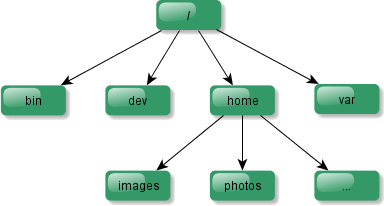
\includegraphics[width=.9\linewidth]{archilin.png}
\textit{Organisation des dossiers sous UNIX}
\end{center}
\end{minipage} \hfill
\begin{minipage}[c]{.49\linewidth}

Quelques dossiers courants sous UNIX:
\begin{itemize}
\item \textit{boot} : fichiers permettant le démarrage de Linux;
\item \textit{etc} : fichiers de configuration;
\item \textit{home} : répertoires personnels des utilisateurs. On en a déjà parlé un peu avant : c'est dans ce dossier que vous placerez vos fichiers personnels, à la manière du dossier Mes documents de Windows.
\end{itemize}
\end{minipage}

\subsection{Droits d’accès}

Les droits d'accès font partie des propriétés d'un fichier. 

Sous UNIX, on peut recenser 3 principaux droits pour un fichier : 
\begin{itemize}
\item le droit en lecture (\textit{r -- read}), qui permet à l'utilisateur de lire le contenu du fichier;
\item le droit en écriture (\textit{w -- write}), qui permet à l'utilisateur d'écrire dans le fichier;
\item le droit d'exécution (\textit{x -- execute}), qui permet à l'utilisateur d'exécuter le fichier.
\end{itemize}

Par ailleurs pour un même ordinateur, il peut exister plusieurs utilisateurs. Ces utilisateurs peuvent de plus appartenir à un groupe.

Ainsi il est possible de distribuer des droits à un utilisateur, à un groupe d'utilisateurs ou à tous les utilisateurs.  

\begin{minipage}[c]{.45\linewidth}
\begin{center}
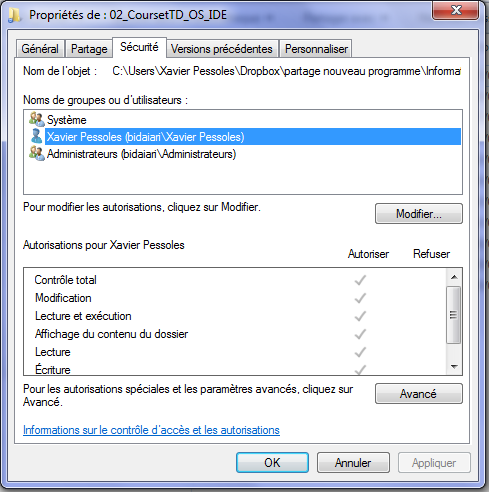
\includegraphics[width=.85\textwidth]{droits_win.png}
\end{center}
\end{minipage}\hfill
\begin{minipage}[c]{.45\linewidth}
\begin{center}
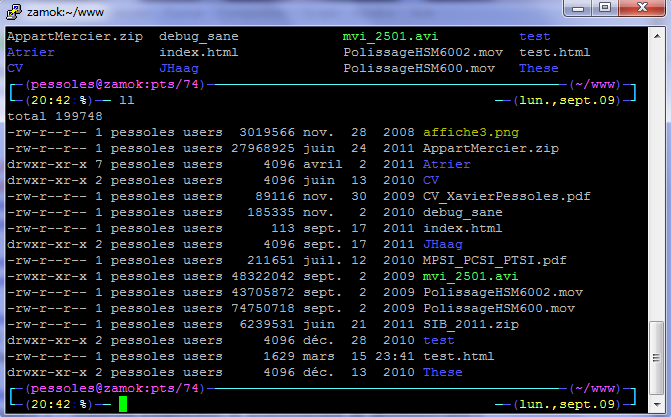
\includegraphics[width=.8\textwidth]{droits_lin.png}
$$
-\underbrace{rw-}_{1}\underbrace{r--}_{2}\underbrace{r--}_{3}
$$
\begin{itemize}
\item 1 : droits pour l'utilisateur pessoles;
\item 2 : droits pour l'utilisateur user;
\item 3 : droits pour le reste du monde.
\end{itemize}
\end{center}
\end{minipage}



\subsection{Notions de réseau}
Les communications Internet se sont développées à partir des années 1990 et ont connu une croissance exponentielle. Le point clé pour permettre de nombreuses communications par réseau internet est d’utiliser des serveurs qui dialoguent entre eux et des clients.
\subsubsection{Client -- Serveur}
Deux ordinateurs sont nécessaires pour créer un réseau.
\begin{defi}[Serveur]
Un serveur est un ordinateur ou un logiciel permettant de fournir des services à un ou plusieurs ordinateurs clients : serveur de fichiers, serveur de courrier électronique, serveur web…
\end{defi}

\begin{defi}[Client]
Un client est un ordinateur ou un logiciel qui demande des services à un serveur. 
\end{defi}

\begin{exemple}~\\


\begin{center}
\begin{tabular}{|l|l|}
\hline
Service installé sur le serveur	& Logiciel installé sur le client utilisant le service \\ \hline
Serveur WEB Apache	&Navigateur (Chrome, Firefox, Iceweasel, Safari,…) \\ \hline
Serveur de diffusion streaming VLC serveur	& Client lecteur de flux video : VLC Client\\ \hline
Serveur de mail : Postfix	&Lecteur de mail : Thunderbird\\ \hline
\end{tabular}
\end{center}
\end{exemple}

Pour les utilisateurs, en général, seul le nom du logiciel « client » est connu.

\subsubsection{Architecture d’un réseau local}
 	 
\begin{center}
\begin{tabular}{p{.47\textwidth}p{.47\textwidth}}
\begin{center}
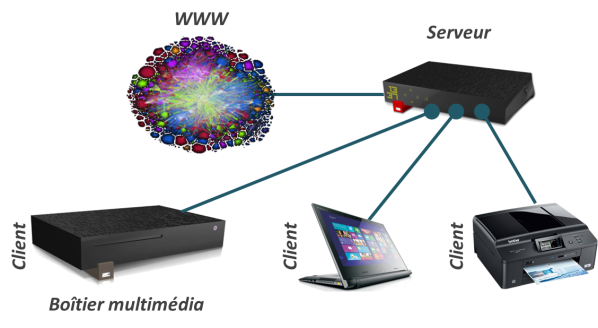
\includegraphics[width=\linewidth]{reseau_01}

Réseau domestique
\end{center} &
\begin{center}
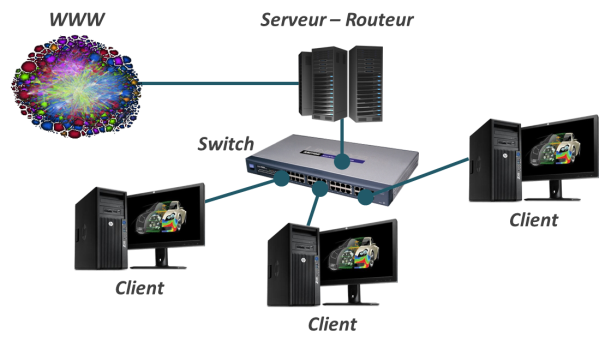
\includegraphics[width=\linewidth]{reseau_02}

Réseau lycéen
\end{center}
\end{tabular}
\end{center}


Dans le cas d’un réseau domestique, le serveur (box) est en fait relié à un serveur du fournisseur d’accès, lui-même relié à internet. Dans ce cas, le serveur joue le rôle de routeur. 

Dans un réseau de lycéen (par exemple), le routeur a la particularité de relier un réseau d’ordinateurs à Internet. Il gère aussi la communication entre les ordinateurs du réseau du lycée.

\section{Applications -- Sources et binaires}
\subsection{Application}
Une application (ou logiciel) est un fichier que l'on peut exécuter afin de satisfaire un besoin (lire un film, ouvre un fichier pdf, naviguer sur internet...). C'est en général un fichier \textbf{binaire}, c'est à dire qu'en général l'utilisateur ne peut pas savoir comment a été codé le logiciel. Il a été produit par l'éditeur de logiciel via un \textbf{compilateur}.

Pour savoir comment une application est codée, il est nécessaire d'en connaître le \textbf{code source}.  Lorsqu'il s'agit d'un logiciel libre, les sources sont disponibles sur Internet. Lorsqu'on travaille chez un éditeur de logiciel, ce code source est aussi accessible. Dans les autres cas, ce code n'est pas accessible. Dans la majorité des cas, l'utilisateur n'a pas besoin de connaître les sources pour utiliser le logiciel. 

Parmi les codes compilés les connus ont peut nommer le \textbf{C} ou le \textbf{C++}. Le langage \textbf{Python} n'a pas besoin d'être compilé pour être exécuté (en apparence). 




\subsection{Python}
\begin{minipage}[c]{.79\linewidth}

Python est un langage de programmation, dont la première version est sortie en 1991. Créé par Guido van Rossum, il a voyagé du Macintosh de son créateur, qui travaillait à cette époque au Centrum voor Wiskunde en Informatica aux Pays-Bas, jusqu'à se voir associer une organisation à but non lucratif particulièrement dévouée, la Python Software Foundation, créée en 2001. Ce langage a été baptisé ainsi en hommage à la troupe de comiques les « Monty Python ».
\end{minipage} \hfill
\begin{minipage}[c]{.2\linewidth}
\begin{center}

\includegraphics[width=.8\textwidth]{monty.jpg}
%\label{}
\end{center}
\end{minipage}

\subsection{À quoi peut servir Python ?}




Python est un langage puissant, relativement facile à apprendre et riche en possibilités. Il est possible d'étendre ses fonctionnalités. On peut aussi appeler des bibliothèques qui aident le développeur à travailler. 

Python permet :
\begin{itemize}
\item de réaliser de petits programmes très simples, appelés scripts, chargés d'une mission très précise sur votre ordinateur;
\item des programmes complets, comme des jeux, des suites bureautiques, des logiciels multimédias, des clients de messagerie…
\item des projets très complexes, comme des progiciels (ensemble de plusieurs logiciels pouvant fonctionner ensemble, principalement utilisés dans le monde professionnel).
\end{itemize}

Voici quelques-unes des fonctionnalités offertes par Python et ses bibliothèques :
\begin{itemize}
\item créer des interfaces graphiques ;
\item faire circuler des informations au travers d'un réseau ;
\item dialoguer d'une façon avancée avec votre système d'exploitation ;
\item ...
\end{itemize}


Python est un langage de programmation interprété, c'est-à-dire comme on l'a spécifié au que les instructions que vous lui envoyez sont « transcrites » en langage machine au fur et à mesure de leur lecture. D'autres langages (comme le C / C++) sont appelés « langages compilés » car, avant de pouvoir les exécuter, un logiciel spécialisé se charge de transformer le code du programme en langage machine. On appelle cette étape la « compilation ». À chaque modification du code, il faut rappeler une étape de compilation.

Les avantages d'un langage interprété sont la simplicité (on ne passe pas par une étape de compilation avant d'exécuter son programme) et la portabilité (un langage tel que Python est censé fonctionner aussi bien sous Windows que sous Linux ou Mac OS, et on ne devrait avoir à effectuer aucun changement dans le code pour le passer d'un système à l'autre). Cela ne veut pas dire que les langages compilés ne sont pas portables, loin de là ! Mais on doit utiliser des compilateurs différents et, d'un système à l'autre, certaines instructions ne sont pas compatibles, voire se comportent différemment.

En contrepartie, un langage compilé se révélera bien plus rapide qu'un langage interprété (la traduction à la volée de votre programme ralentit l'exécution), bien que cette différence tende à se faire de moins en moins sentir au fil des améliorations. De plus, il faudra installer Python sur le système d'exploitation que vous utilisez pour que l'ordinateur puisse comprendre votre code.



\newpage

%
%\section{Architecture de base d'un ordinateur}
%\subsection{Introduction}
%L'informatique, contraction d'information et automatique, est la science du traitement de l'information. Apparue au milieu du 20ème siècle, elle a connu une évolution extrêmement rapide. À sa motivation initiale qui était de faciliter et d'accélérer le calcul, se sont ajoutées de nombreuses fonctionnalités, comme l'automatisation, le contrôle et la commande de processus, la communication ou le partage de l'information.
%Ce cours expose les principes de base du traitement programmé de l’information. La mise en œuvre de ces systèmes s’appuie sur :
%\begin{itemize}
%\item le matériel (hardware), qui est l’objet de ce cours, correspond à l’aspect concret du système : unité centrale, mémoire, organes d’entrées-sorties, etc…
%\item le logiciel (software) correspond à un ensemble d’instructions, appelé programme, qui sont contenues dans les différentes mémoires du système et qui définissent les actions effectuées par le matériel.
%\end{itemize}
%
%
%\subsection{Constitution d’un ordinateur du laboratoire}
%
%
%\begin{figure}[h]
%\begin{minipage}[c]{.49\linewidth}
%\begin{center}
%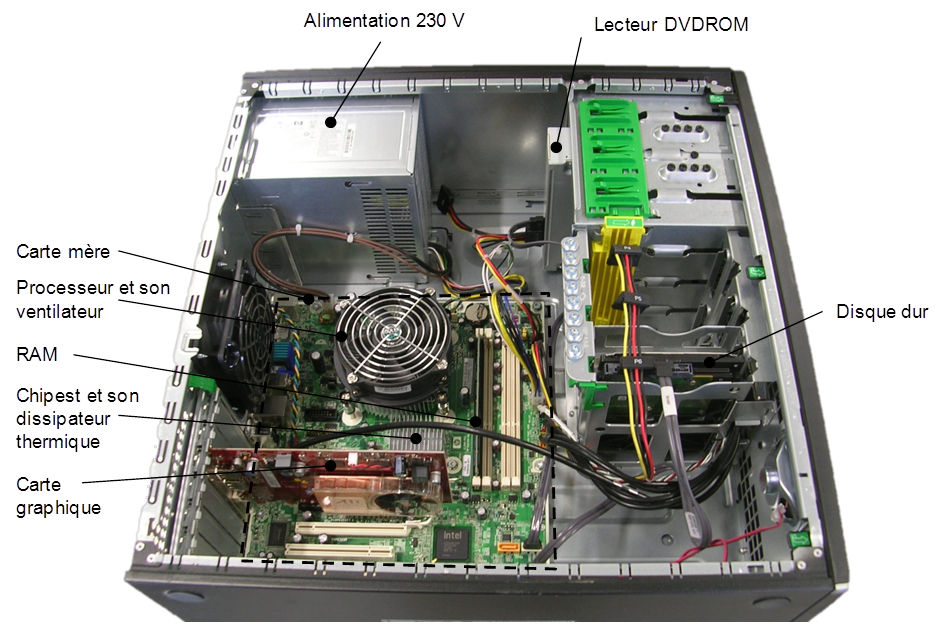
\includegraphics[width=.99\textwidth]{ordi1.png}
%\label{}
%\end{center}
%\end{minipage} \hfill
%\begin{minipage}[c]{.49\linewidth}
%\begin{center}
%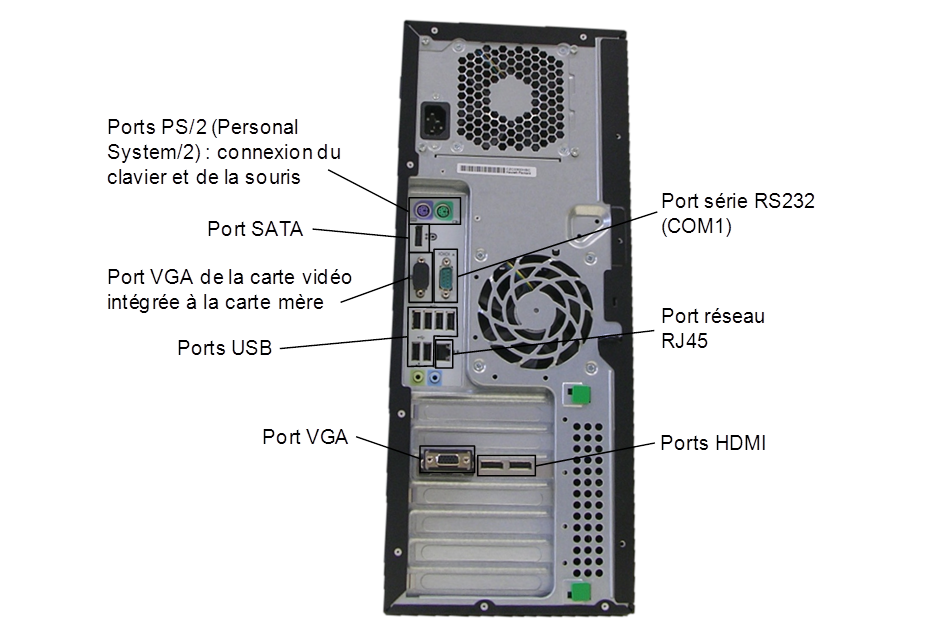
\includegraphics[width=.99\textwidth]{ordi2.png}
%\label{}
%\end{center}
%\end{minipage}
%\end{figure}
%
%\subsection{Modèle de Von Neumann}
%
%Pour pouvoir exécuter des algorithmes arbitraires, les ordinateurs actuels sont tous bâtis
%autour du même modèle architectural théorique, l’architecture de Von Neumann, même
%si la mise en oeuvre pratique est un peu plus complexe.
%
%Le premier ordinateur électronique fut l’ENIAC
%(dont le but était de calculer des tables indiquant les paramètres de tir d’une batterie d’artillerie
%en fonction de la distance de l’objectif, du vent, etc.) dont la construction démarra
%en 1943. 
%
%\begin{figure}[h]
%\begin{minipage}[c]{.49\linewidth}
%
%Son architecture a été décrite dans un rapport de John Von Neumann en 1945 et
%est depuis appelée «~architecture de Von Neumann~». Depuis près de 70 ans, à quelques variations
%près, cette  architecture sert de base à la plupart des systèmes à microprocesseur actuel. Elle est composée des éléments suivants :
%\begin{itemize}
%\item d'une mémoire vive ;
%\item d'un processeur qu'on peut conceptuellement décomposer en une unité de contrôle et
%une unité de calcul arithmétique et logique ;
%\item de dispositifs périphériques, appelés simplement périphériques ;
%\item d'un canal de communication entre la mémoire, le processeur et les périphériques, appelé
%le bus.
%\end{itemize}
%
%\end{minipage} \hfill
%\begin{minipage}[c]{.49\linewidth}
%\begin{center}
%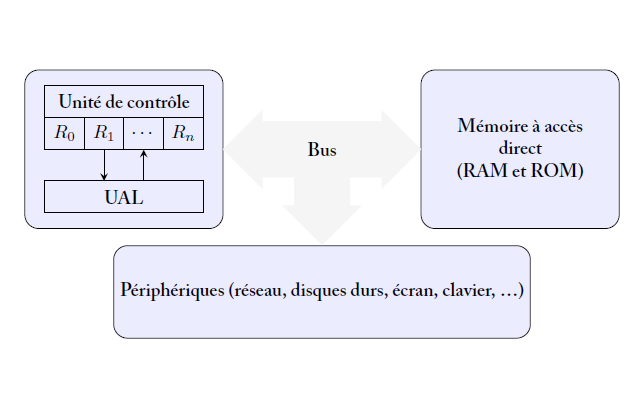
\includegraphics[width=.99\textwidth]{von.png}
%\caption{Architecture de Von Neumann}
%\label{}
%\end{center}
%\end{minipage}
%\end{figure}
%
%
%
%
%\section{La carte mère}
%La carte mère constitue le c\oe{}ur d'un ordinateur. Elle est abritée par une tour sur un ordinateur de bureau ou par le boîtier sous le clavier dans un ordinateur portable. Elle est équipée de divers connecteurs permettant de brancher, l'alimentation, le(s) processeur(s)
%les ventilateurs, 
%la mémoire vive, 
%le disque dur (et autres disques), 
%la carte réseau, 
%la carte son, 
%la carte graphique lorsque celle-ci n'est pas intégrée, 
%l(es)'écran(s), 
%le clavier,  
%la souris, 
%les autres périphériques (imprimantes, scanner, lecteurs multimédias, téléphones ...).
%
%
%
%\subsection{Cartes mères}
%
%La plupart des cartes mères utilisées dans les ordinateurs de bureau sont au format ATX. Elles imposent donc certaines dimensions pour le boîtier (tour). Elles assurent la liaison avec tous les composants.
%
%\begin{center}
%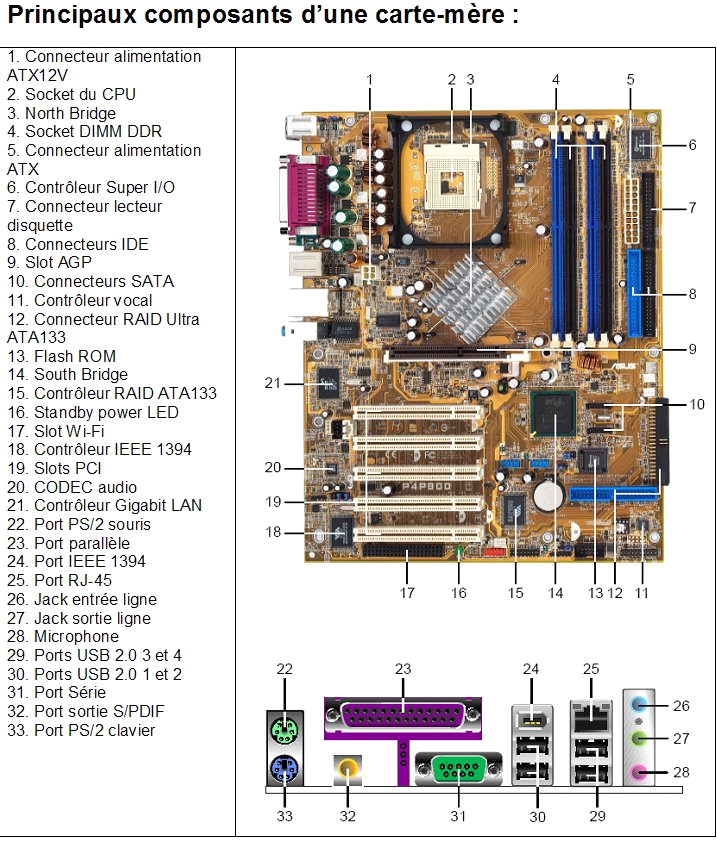
\includegraphics[width=.7\textwidth]{carte_mere_2.png}
%\end{center}
%
%
%
%
%\begin{figure}[h]
%\begin{minipage}[c]{.49\linewidth}
%
%Le fonctionnement de la carte mère est assuré par des chipsets (ensemble de composants électroniques) qui permettent l'échange des données entre les différents composants branchés. Le northbridge gère les composants branchés <<rapides>> (la mémoire cache par exemple). Le southbridge est le chipset permettant la gestion des composants <<lents>> (comme le disque dur). 
%
%Le flux des informations est cadencé par une horloge permettant leur synchronisation. Cette horloge est alimentée de façon permanente par une pile. 
%
%Le BIOS (\textit{Basic Input/Output System}) est un logiciel directement installé sur la carte mère qui permet d'assurer la communication entre le matériel et le système d'exploitation. 
%
%\end{minipage} \hfill
%\begin{minipage}[c]{.49\linewidth}
%\begin{center}
%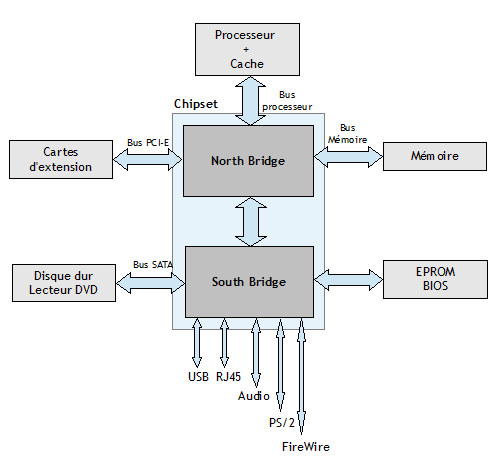
\includegraphics[width=.9\textwidth]{carte.png}
%\label{}
%\end{center}
%\end{minipage}
%\end{figure}
%
%Sur la carte mère, la communication entre les différents composants est assurée par des bus :
%\begin{itemize}
%\item le bus système relie le micorprocesseur au chipset;
%\item le bus mémoire relie le chipset à la mémoire vive;
%\item le bus d'extension relie le chipset aux connecteurs d'entrée -- sortie.
%\end{itemize}
%
%\subsection{CPU (\textit{Central Processing Unit})}
%
%
%\noindent\begin{minipage}[c]{.65\linewidth}
%Le CPU aussi appelé processeur ou microprocesseur est le cerveau du PC. Sa puissance dépend du nombre de cœurs du processeur, de la taille de sa mémoire cache, de l'architecture du processeur et de sa fréquence.
%
%La fréquence du CPU s'exprime en MHz ou en GHz. C'est une valeur à laquelle les utilisateurs
%attachent le plus d'importance mais d'autres paramètres en déterminent les performances.
%Dans un ordinateur, non seulement les données traitées sont discrètes, mais le déroulement
%des opérations se fait aussi selon un temps discrétisé.
%\end{minipage}\hfill
%\begin{minipage}[c]{.3\linewidth}
%\begin{center}
%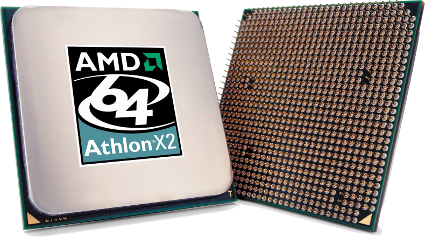
\includegraphics[width=.8\textwidth]{cpu_amd_p.png}
%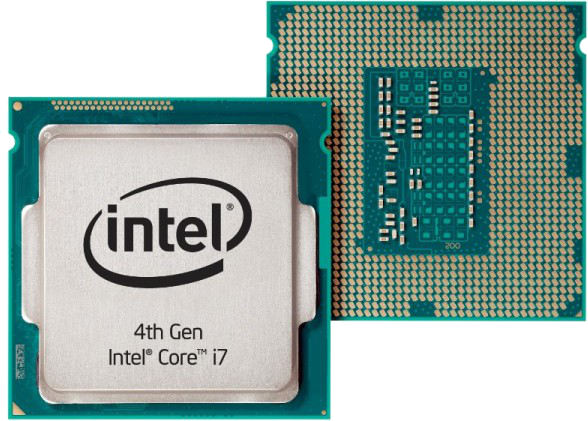
\includegraphics[width=.8\textwidth]{cpu_intel.png}
%\end{center}
%\end{minipage}
%
%\vspace{.25cm}
%
%La mémoire cache permet au processeur d'avoir à sa disposition une mémoire d'accès rapide mais dont la capacité est relativement limitée. 
%
%
%Une horloge, le plus souvent calibrée à l'aide d'oscillateurs à quartz, émet régulièrement une suite d'impulsions, comme un métronome, qui sert à scander les opérations. Le temps d'un
%cycle, ou période de l'horloge, est une caractéristique des processeurs : par exemple 1 Ghz,
%c'est-à-dire une impulsion tous les milliardièmes de secondes.
%
%L'efficacité du CPU dépend aussi de son architecture interne. Les processeurs actuels
%traitent plusieurs instructions par cycle. Ces traitements se font en parallèle grâce
%notamment à la technique du double pipeline d'instructions, ce qui leur permet d'effectuer
%deux ou trois instructions par cycle.
%
%Le rôle de la mémoire cache est d'autant plus important que la vitesse du CPU est élevée par
%rapport à celle de la mémoire RAM. Cet écart ne cesse d'augmenter car l'évolution des CPU est bien plus rapide que celle des
%mémoires. La mémoire cache coûte cher. Sa taille explique souvent la différence de prix
%entre les processeurs.
%
%L'augmentation des fréquences a atteint des limites aux environs de 4 GHz. La seule façon
%d'augmenter encore les performances est maintenant de multiplier les cœurs sur la même
%puce.
%
%
%Un ensemble de fils appelé bus partent du CPU et permettent de le connecteur aux autres composants du système.
%Le CPU est constitué essentiellement de trois parties :
%\begin{itemize}
%\item l'unité de commande qui cherche les instructions en mémoire, les décode et coordonne le
%reste du processeur pour les exécuter. Une unité de commande élémentaire se compose
%essentiellement d'un registre d'instruction et d'une unité <<décodeur / séquenceur>>;
%\item l'Unité Arithmétique et Logique (UAL) exécute les instructions arithmétiques et logiques
%demandées par l'unité de commande. Les instructions peuvent porter sur un ou plusieurs
%opérandes. La vitesse d'exécution est optimale quand les opérandes se situent dans les
%registres plutôt que dans la mémoire externe au processeur;
%\item les registres sont des cellules mémoire interne au CPU. Ils sont peu nombreux mais d'accès
%très rapide. Ils servent à stocker des variables, les résultats intermédiaires d'opérations
%(arithmétiques ou logiques) ou encore des informations de contrôle du processeur.
%
%\end{itemize}
%
%
%\begin{center}
%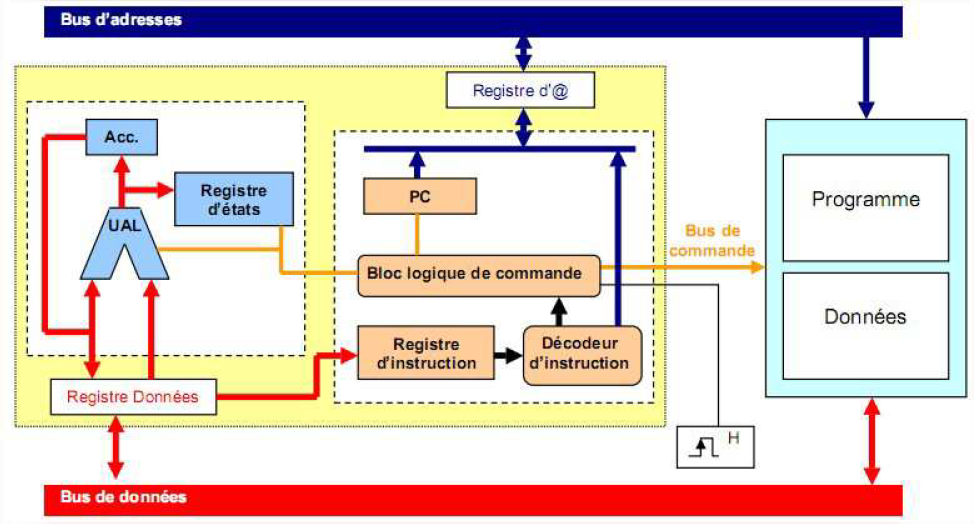
\includegraphics[width=.85\textwidth]{archi_cpu}
%\end{center}
%
%La structure des registres varie d'un processeur à l'autre. C'est ce qui fait que chaque type de CPU a un jeu d'instruction qui lui est propre. Leurs fonctions de base sont néanmoins
%semblables et tous les processeurs possèdent en gros les mêmes catégories de registres :
%\begin{itemize}
%\item l'accumulateur est principalement destiné à contenir les données qui doivent être
%traitées par l'UAL;
%\item les registres généraux servent au stockage de résultats intermédiaires;
%\item les registres d’adresse servent à confectionner des adresses de données
%particulières : ce sont, par exemples, les registres de base et d'index qui permettent
%entre autres d'organiser les données en mémoire comme des tables indicées.
%\item le registre d'instruction (RI) contient le code de l'instruction qui est traitée par le
%décodeur / séquenceur;
%\item le compteur ordinal (CO) ou Program Counter (PC) contient l'adresse de la
%prochaine instruction à exécuter. En principe, ce registre ne cesse de compter. Il
%génère les adresses des instructions à exécuter les unes à la suite des autres.
%Certaines instructions demandent quelquefois de changer le contenu du compteur
%ordinal pour faire une rupture de séquence c'est à dire un saut ailleurs dans le
%programme.
%\end{itemize}
%
%
%\subsection{Les bus}
%
%En informatique, le terme bus désigne un ensemble de fils support de l'information et organe de communication entre différents composants.Il existe deux grands types de bus :
%\begin{itemize}
%\item le bus série : il comporte plusieurs fils, dont la masse (référence de potentiel), le fil de données, le fil d'horloge. Les données sont transmises en série;
%\item le bus parallèle : il comporte un fil de masse, un fil d'horloge, et $n$ fils de données pour un bus $n$ bits ; les données sont transmises en parallèle.
%\end{itemize}
%
%Par ailleurs, des bus sont intégrés dans des puces. Par exemple, dans les microprocesseurs, les différents constituants communiquent entre eux par des bus parallèles.
%	
%Sur la carte mère sont intégrés différents bus parallèles que l'on peut même parfois distinguer. Ces bus permettent de relier les différents constituants entre eux afin qu'ils communiquent. On retrouve des bus d'adresses, de données et de contrôle.
%
%Entre la carte mère et les différents périphériques (disque dur par exemple), on utilise de plus en plus des bus séries. Ainsi, après le tout IDE, bus parallèle qui a été massivement utilisé dans les ordinateurs grand public, le bus SATA est de plus en plus utilisé. .
%
%Le bus SATA ou S-ATA (\textit{Serial ATA}) a été conçu afin de pallier aux problèmes constatés à haute fréquence sur le bus IDE encore appelé Parallel ATA.
%Plusieurs normes SATA ont été développées. 
%
%\begin{center}
%\begin{tabular}{|c|c|}
%\hline
%Norme & Débit ($Mo/s$) \\
%\hline
%SATA I & 187,5 \\ \hline
%SATA II & 375 \\ \hline
%SATA III & 750 \\ \hline
%\end{tabular}
%\end{center}
%
%Cette technologie présente des débits bien plus importants que les disques durs mécaniques  (60 Mo/s au mieux) mais va en revanche bien s'adapter aux débits des SSD qui commencent à avoisiner les 500 Mo/s.
%
%
%\section{Les mémoires}
%\subsection{Mémoire de masse}
%\subsubsection{Le disque-dur magnétique}
%
%
%\paragraph*{Description}
%\begin{minipage}[c]{.65\linewidth}
%Le disque dur (\textit{HDD -- Hard Disk Drive}) doit son nom à sa technologie à l'époque où existaient encore les disques souples, ou disquettes.
%
%Le disque dur est alimenté par un connecteur Molex ou par adaptateur de courant SATA. Ces connecteurs sont reliés à l'alimentation du PC. 
%
%La capacité des disques durs actuels atteint les 4 To (téraoctet). Lorsqu'ils sont connectés en SATA, le débit oscille entre 30 et 60 \textit{Mo/s} et peut atteindre les 600 \textit{Mo/s}. Enfin, pour améliorer les performances d'accès aux données, ils possèdent une mémoire cache pouvant aller jusqu'à 128 \textit{Mo} sur laquelle sont stockées les informations fréquemment utilisées. 
%
%\end{minipage}\hfill
%\begin{minipage}[c]{.3\linewidth}
%\begin{center}
%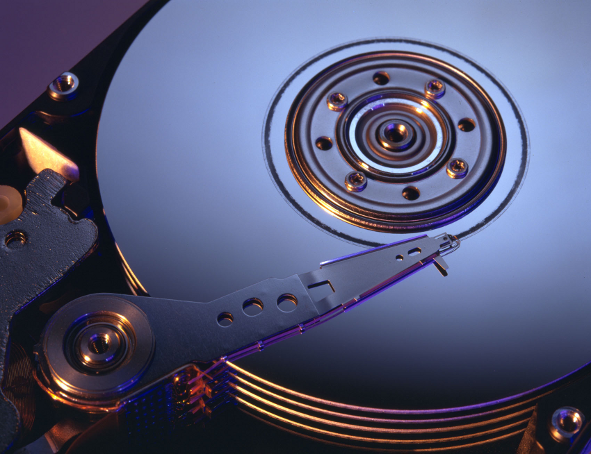
\includegraphics[width=.7\textwidth]{dd_1_p.png}
%\end{center}
%\end{minipage}
%
%
%\paragraph*{Principe de fonctionnement}
%
%
%\begin{minipage}[c]{.6\linewidth}
%Un disque dur est composé de disques rigides et paramagnétiques (en aluminium, en verre ou en céramique) recouverts d'une couche magnétique et d'un film protecteur. Ces plateaux sont entraînés par un moteur électrique dont la fréquence de rotation est fixe. La fréquence de rotation peut atteindre les 15 000 \textit{tr/min}. Un bras, sur lequel sont fixées les têtes de lecture -- écriture, est aussi motorisé pour atteindre les différentes parties du disque. La distance entre les têtes et les plateaux est de l'ordre de 10 \textit{nm}. Elle est maintenue par un coussin d'air formé par la rotation des disques. 
%\end{minipage} \hfill
%\begin{minipage}[c]{.35\linewidth}
%\begin{center}
%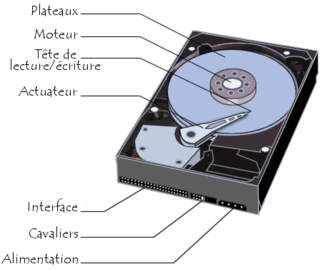
\includegraphics[width=.9\textwidth]{dd_comp.png}
%\end{center}
%\end{minipage} 
%
%Les têtes de lecture -- écriture sont inductives et permettent de générer un champ magnétique dans deux sens opposés permettant de polariser la couche magnétique du disque. Ainsi, en mode lecture les changements de polarité sont transcrits par un convertisseur analogique numérique (CAN) en bits (0 ou 1).
%
%Les données sont organisées en pistes concentriques, les données les plus rapidement accessibles étant celles situées sur le disque extérieur. Chaque piste est divisée en secteurs (d'un minimum de 512 octets). Enfin, on appelle cylindre l'ensemble de données situé sur une même piste mais sur un plateau différent. 
%
%
%%
%%\begin{center}
%%\begin{tabular}{|c|c|c|c|c|}
%%\hline
%%Capacité & Année & Fabriquant & Modèle & Taille \\ \hline
%%5 Mo & 1956 & IBM & 305 RAMAC & 24''\\ \hline
%%28 Mo & 1962 & IBM & Modèle 1301 & \\ \hline
%%1.02 Go & 1982 & Hitachi & H8598 & 14''\\ \hline
%%25 Go & 1998 & IBM & Deskstar 25 GP & 7,0'' \\ \hline
%%500 Go & 2005 & Hitachi & & 3,5''\\ \hline
%%1 To & 2007 & Hitachi & Deskstar 7K1000 & 3,5''\\ \hline
%%2 To & 2009 & Western Digital & Caviar Green WD20EADS & 3,5''\\ \hline
%%3 To & 2010 & Seagate & & 3,5''\\ \hline
%%4 To & 2011 & Hitachi & 7K4000 & 3,5''\\
%%\hline
%%\end{tabular}
%%
%%\textit{Capacité actuelle des ordinateurs}
%%\end{center}
%
%
%
%
%
%\subsubsection{Disques dur SSD -- \textit{Solid State Drive}}
%
%
%
%
%\begin{center}
%\begin{tabular}{|l|l|l|}
%\hline
%\textbf{Caractéristiques} & \textbf{Disque dur mécanique} & \textbf{SSD} \\ \hline
%Temps d'accès & En moyenne 12ms & 0.1ms \\ \hline
%Poids & De 400g à 700g & Quelques dizaines de grammes \\ \hline
%Consommation en veille & De l'ordre du Watt & 100 mW \\ \hline
%Consommation en activité & 4W environ & 900 mW \\ \hline
%Bruit  & En moyenne 40 dB & 0 dB\\ \hline
%\end{tabular}
%\end{center}
%
%Les performances du SSD sont supérieures à celles des disques durs classiques. Deux critères penchent néanmoins en sa défaveur. D'une part le prix du Go est presque 10 fois plus élevé 
%que pour un disque dur mécanique. D'autre part, certaines technologies de SSD présentent l'inconvénient d'être limité en nombre de cycles d'écriture -- lecture.
%
%\subsubsection{Disques durs hybrides}
%Le disque dur hybride est l'exact compromis entre un disque dur mécanique « conventionnel » et un disque dur SSD. C'est un disque dur mécanique auquel on a adjoint un volume mémoire flash conséquent (quelques Go), ou du moins suffisant pour que l'effet s'en ressente sur son utilisation en comparaison d'un disque dur mécanique. L'intérêt est une réduction très nette du prix du disque dur pour des performances accrues tout en limitant les risques de pertes de mémoire sur le SSD de technologie encore limitée en nombre de cycles mémoires.
%
%
%Actuellement, l'un des disques de plus grande capacité est le Seagate Momentus XT 7200 Hybrid SSD 750Go SLC 8Go NAND Flash. On trouve également dans la marque Western Digital le WD Black SSHD, 1 To en stockage classique et 24 Go de mémoire NAND Flash.
%
%
%
%\subsection{La mémoire vive}
%
%\noindent \begin{minipage}[c]{.6\linewidth}
%Les mémoires de type RAM (\textit{Random Access Memory} -- Mémoire à accès aléatoire) sont des mémoires dites volatiles, c'est-à-dire dont le contenu disparaît en absence d'alimentation.
%Elles sont utilisées bien-sûr dans les PC et autres ordinateurs personnels comme mémoire de travail du système. Les mémoires Cache sont également des RAM.
%
%
%\end{minipage}
%\begin{minipage}[c]{.3\linewidth}
%\begin{center}
%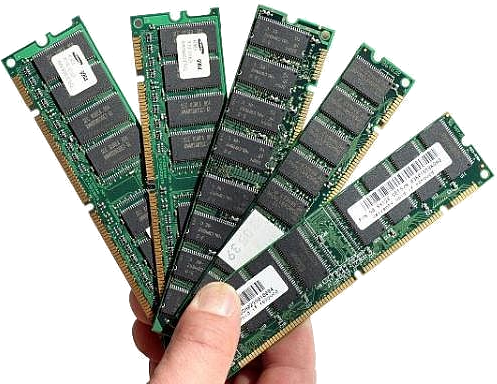
\includegraphics[width=.9\textwidth]{ram.png}
%\end{center}
%\end{minipage}
%
%Une autre grosse différence avec les ROM concerne la fréquence de fonctionnement (ou le temps d'accès) des RAM. La fréquence de fonctionnement de la RAM en général est beaucoup plus élevée que pour la ROM. La raison principale en est une différence essentielle de structure.
%
%Le temps d'accès des mémoires RAM est de quelques nanosecondes pour une capacité de l'ordre de quelques Go.
%
%
%\subsection{La mémoire ROM (« mémoire morte »)}
%
%
%\begin{figure}[h]
%\begin{minipage}[c]{.49\linewidth}
%
%Historiquement, les ROM (\textit{Read Only Memory}-- Mémoire en lecture seule) étaient effectivement des mémoires en lecture seule. Leur grosse différence avec les RAM est que leur contenu perdure malgré l'absence d'alimentation. Elles seront donc par exemple très utiles pour stocker les programmes et informations de démarrage (BIOS, Setup CMOS, le POST (Power On Self Test)). Mais leurs fonctions ne se limitent pas à celle-ci.
%
%\end{minipage} \hfill
%\begin{minipage}[c]{.49\linewidth}
%\begin{center}
%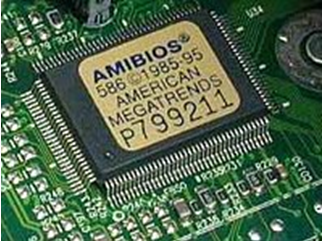
\includegraphics[width=.5\textwidth]{ROM.png}
%\label{}
%\end{center}
%\end{minipage}
%\end{figure}
%Actuellement, on utilise le plus souvent des EEPROM ( Electrically Erasable Programmable ROM ).
%
%Si l'appellation ROM désigne le plus souvent les puces mémoires, on ne peut oublier :
%\begin{itemize}
%\item les CD-ROM, les DVD-ROM
%\item les Bluray sont des ROM
%\item les disques durs sont des ROM ( car non volatiles )
%\item les SSD sont des ROM
%\item les clefs USB sont des ROM ( mémoire flash )
%\end{itemize}
%
%Le temps d'accès pour une puce ROM du type de celles utilisées pour le BIOS ou la CMOS est de l'ordre de quelques dizaine de nanosecondes. Leur capacité varie selon le support considéré (puce, SSD, \textit{etc.}).
%

%\section{Communication}
%
%
%
%\section{Notion de système d'exploitation}
%
%\subsection{Introduction}
%
%Le système d'exploitation (\textit{Operating System -- OS}) est un programme chargé en mémoire vive dès le démarrage de l'ordinateur et qui reste en mémoire jusqu'à son extinction. 
%
%Pour les \textbf{ordinateurs monoprocesseur} ce programme a pour but de donner l’illusion que l’ordinateur est multitâche lorsque plusieurs applications sont lancées en même temps. Pour cela, il stocke en mémoire les différentes applications que l’on veut exécuter. Il lance l’exécution d’une première application. Dès qu’il se produit une entrée-sortie ou, à défaut, lorsqu’un certain temps est écoulé (de l’ordre de la centaine de millisecondes), le noyau du système d’exploitation reprend la main et lance l’exécution d’une autre application. En pratique, le temps d’exécution d’une tâche dépasse rarement la dizaine de millisecondes.
%
%Pour les \textbf{ordinateurs multiprocesseurs} ce programme a pour but de gérer les accés de chacun des processeurs à la mémoire et aux périphériques, ce qui permet
%effectivement que l’ordinateur exécute plusieurs instructions à la fois. Les fabricants
%de processeurs proposent même maintenant des processeurs qui contiennent en fait plusieurs
%c\oe{}urs (dualcore, quadricore), c’est-à-dire que plusieurs processeurs (unité arithmétique
%et logique et unité de contrôle) ont été regroupés sur un seul processeur.
%
%Par ailleurs l'OS permet de manière générale de gérer l'organisation des données sur le disque dur ainsi que leur droit d'accès. Il gère aussi les différentes ressources et sert de garde-fou en cas de tentative de mauvaise utilisation des ressources de l'ordinateur.
%
%Pour finir, l'OS permet à un ou plusieurs utilisateurs de s'identifier leur permettant ainsi d'utiliser un seul ordinateur sans nécessairement partager les données et les programmes. 
%
%
%Il existe essentiellement deux grandes familles de systèmes d’exploitation. 
%
%\begin{minipage}[c]{.7\linewidth}
%Les systèmes d’exploitation de la famille Microsoft-Windows qui sont en situation de quasi-monopole sur les \textbf{ordinateurs personnels} (ils en équipent près de 90\%)
%
%\end{minipage} \hfill
%\begin{minipage}[c]{.25\linewidth}
%\begin{center}
%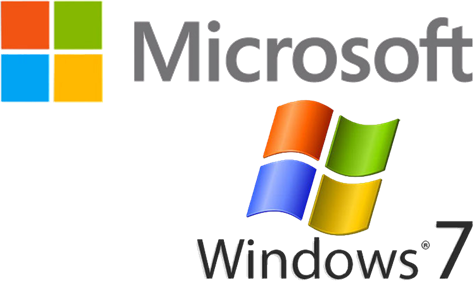
\includegraphics[width=.9\textwidth]{ms}
%\end{center}
%\end{minipage} 
%
%\begin{minipage}[c]{.7\linewidth}
%Les systèmes d’exploitation issus d’Unix (Mac OS X, iOS, GNU/Linux, Android, FreeBSD, NetBSD). Dans tous les domaines, sauf celui des ordinateurs personnels, les systèmes issus d’Unix sont majoritaires.  Linux s’est imposé comme un système universel puisqu’il équipe aussi bien les téléphones portables (Android) que les boîtiers prêtés par les fournisseurs d’accès à Internet, les ordinateurs personnels (Ubuntu/GNU Linux), les serveurs web et les supercalculateurs (plus de 90\% des calculateurs du TOP 500).
%
%\end{minipage} \hfill
%\begin{minipage}[c]{.25\linewidth}
%\begin{center}
%
\includegraphics[width=.9\textwidth]{genlin}
%\end{center}
%\end{minipage} 
%
%Il est possible d'installer plusieurs systèmes d'exploitation sur une même machine: double boot. Il est aussi possible d'émuler un système d'exploitation dans un autre système d'exploitation.
%
%\subsection{Petit historique}
%
%\begin{center}
%\begin{tabular}{m{1cm}m{10cm}m{6cm}}
%\textbf{1969} & 
%Origines de UNIX. & 
%\begin{center}
%%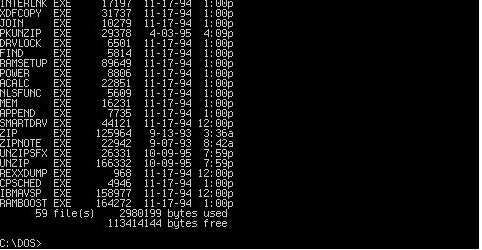
\includegraphics[width=7cm]{dos.jpg}
%\end{center}
%\end{tabular}
%
%\begin{tabular}{m{1cm}m{10cm}m{6cm}}
%\textbf{1984} & 
%Sortie du premier OS de Microsoft : MS-DOS. & 
%\begin{center}
%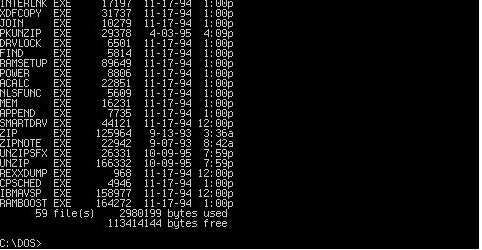
\includegraphics[width=6cm]{dos.jpg}
%\end{center}
%\end{tabular}
%
%\begin{tabular}{m{1cm}m{10cm}m{6cm}}
%\textbf{1984} & 
%Richard Stallman\footnotemark[1] crée le projet GNU dans le but de développer un OS basé sur Unix, mais libre. & 
%\begin{center}
%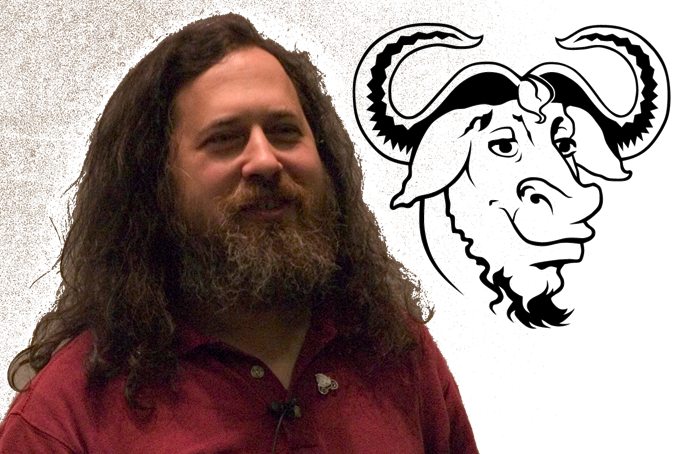
\includegraphics[width=6cm]{richard.png}
%\end{center}
%\end{tabular}
%
%\begin{tabular}{m{1cm}m{10cm}m{6cm}}
%\textbf{1991} & 
%
%Linus Torvalds\footnotemark[2] entreprend de créer sur son temps libre son propre système d'exploitation. Ce système a pris le nom de Linux (contraction de Linus et Unix). Ce projet est complémentaire du projet GNU : tandis que Richard Stallman créait les programmes de base (programme de copie de fichier, de suppression de fichier, éditeur de texte), Linus s'est lancé dans la création du « cœur » d'un système d'exploitation : le noyau.
% & 
%\begin{center}
%
\includegraphics[width=3cm]{linux.png}
%\end{center}
%\end{tabular}
%
%\end{center}
%
%\footnotetext[1]{Chercheur en intelligence artificielle au MIT.}
%\footnotetext[2]{\'Etudiant de l'Université de Helsinki (Finlande).}
%
%
%%
%%
%%\begin{figure}[h]
%%\begin{minipage}[c]{.49\linewidth}
%%\begin{center}
%%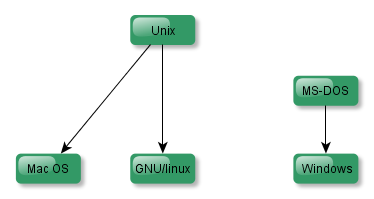
\includegraphics[width=.99\textwidth]{origine.png}
%%\caption{Origine des systèmes d'exploitation}
%%\label{}
%%\label{essai1}
%%\end{center}
%%\end{minipage} \hfill
%%\begin{minipage}[c]{.49\linewidth}
%%Le projet GNU (programmes libres) et Linux (noyau d'OS) ont fusionné pour créer GNU/Linux.
%%Théoriquement, on doit donc parler de GNU/Linux. C'est toutefois un peu difficile à écrire et prononcer, et par abus de langage, on dit souvent juste « Linux ». 
%%\newline\newline
%%Mac OS X est lui aussi basé sur Unix. En revanche, MS-DOS et Windows sont complètement à part.
%%\end{minipage}
%%\end{figure}
%%
%
%
%
%
%\begin{rem}
%Un programme libre est un programme dont on peut avoir le code source, c'est-à-dire la « recette de fabrication ». Au contraire, Windows est un OS propriétaire dont le code source est conservé par Microsoft. On ne peut donc pas le modifier ou regarder comment il fonctionne à l'intérieur.
%
%Un programme libre est donc la plupart du temps un programme gratuit. Mais c'est aussi un programme qu'on a le droit de copier, modifier, redistribuer. On dit aussi souvent que le programme est « Open Source » car son code source est ouvert ; tout le monde peut le voir.
%
%Il existe quelques légères différences entre un programme « Open Source » et un programme « libre », mais nous n'entrerons pas dans les détails ici.
%\end{rem}
%
%
%
%\begin{rem}
%\textit{Les distribution GNU/Linux}
%
%Une distribution est un ensemble de logiciels articulés autour d'un noyau. GNU/Linux comprend un grand nombre de distributions. Elles diffèrent par la méthode d'installation, la gestion des programmes, la méthode pour installer des programmes. Attention, le terme distribution est différent du terme logiciel. De manière générale, un logiciel libre est installable sur n'importe quelle distribution. Dans le cas le plus défavorable, il sera nécessaire de \textbf{compiler} le logiciel.
%
%
%%
%%Pour simplifier la vie des utilisateurs et leur permettre de faire un choix, différentes distributions de Linux ont été créées. C'est un concept qui n'existe pas vraiment sous Windows. C'est un peu comme la différence entre Windows 7 Familial et Windows 7 Professionnel, mais cela va bien plus loin que ça.
%%
%%Voici ce qui peut différer d'une distribution à l'autre :
%%\begin{itemize}
%%\item l'installation : elle peut être très simplifiée comme très compliquée ;
%%\item la gestion de l'installation des programmes. Si elle est bien faite et centralisée, elle peut rendre l'installation de nouveaux logiciels plus simple que sous Windows, comme nous le verrons plus loin !
%%\item les programmes préinstallés sur l'ordinateur (Windows est par exemple livré avec Internet Explorer et Windows Media Player).
%%\end{itemize}
%%En fait, une distribution est en quelque sorte l'emballage de Linux. Le cœur, lui, reste le même sur toutes les distributions.
%%
%%Il existe un grand nombre de distributions Linux différentes:
%%\begin{itemize}
%%\item Slackware : une des plus anciennes distributions de Linux. Elle existe encore aujourd'hui !
%%\item Mandriva : éditée par une entreprise française, elle se veut simple d'utilisation ;
%%\item Red Hat : éditée par une entreprise américaine, cette distribution est célèbre et très répandue, notamment sur les serveurs ;
%%\item SuSE : éditée par l'entreprise Novell ;
%%\item Debian : la seule distribution qui soit gérée par des développeurs indépendants plutôt que par une entreprise. C'est une des distributions les plus populaires.
%%\end{itemize}
%%
%%
%%
%%
%%\begin{figure}[h]
%%
%%\begin{minipage}[c]{.49\linewidth}
%%Prenons l'exemple de la distribution Debian.
%%Les autres distributions sont gérées par des entreprises, ce qui ne les empêche pas d'être « Open Source » et gratuites, même si nous pouvons également les acheter pour avoir droit à une assistance (hotline…). Debian est donc la seule distribution éditée par des particuliers bénévoles à travers le monde. 
%%Debian a tellement de succès que de nombreuses distributions sont basées sur Debian, ce sont donc des… distributions de distributions. 
%%Ubuntu est une des distributions les plus populaires à l'heure actuelle.
%%\end{minipage} \hfill
%%\begin{minipage}[c]{.49\linewidth}
%
%%\end{minipage}
%
%\begin{center}
%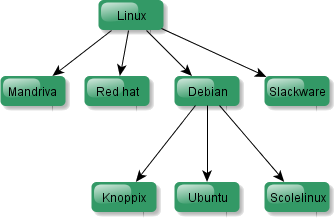
\includegraphics[width=.6\textwidth]{distrib.png}
%
%\textit{Différentes distributions GNU/Linux}
%
%\end{center}
%
%\end{rem}
%
%
%
%
%\subsection{À quoi ressemble Linux ?}
%
%
%%\subsubsection{En mode console}
%
%%\begin{figure}[h]
%\begin{minipage}[c]{.49\linewidth}
%Une des réticences à l'utilisation d'une distribution GNU/Linux est le mode console. 
%
%Ce mode de fonctionnement peut paraître effrayant et peu accessible pour un utilisateur novice. Cependant, le mode console permet de faire une grande partie des opérations faisable avec la souris ce qui, avec l'expérience, améliore l'efficacité de l'utilisateur.
%\end{minipage} \hfill
%\begin{minipage}[c]{.49\linewidth}
%\begin{center}
%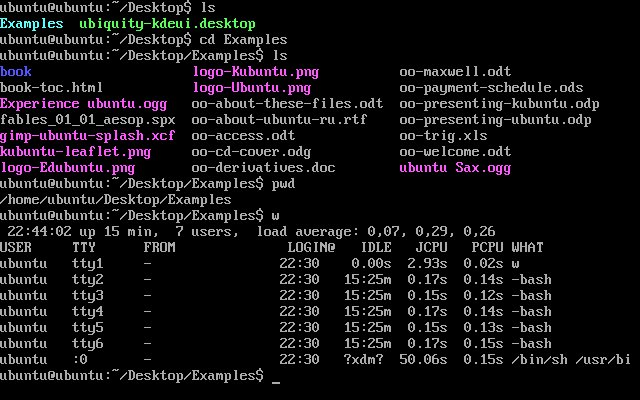
\includegraphics[width=.9\textwidth]{commande.jpg}
%\end{center}
%\end{minipage}
%%
%%\begin{warn}
%%\textsc{ATTENTION}
%%
%%Ce serait une lourde erreur de croire que l'utilisation des interprètes de commandes en mode text  est
%%dépassée. Leur usage demande certes plus de travail au départ que l'utilisation d'un shell
%%graphique. Mais c'est l'une des façons les plus productives de faire exécuter des tâches à un
%%ordinateur et pour l'administrateur d'un système, c'est bien souvent un outil indispensable.
%%\end{warn}
%%\end{minipage}
%%\end{figure}
%
%%\subsubsection{En mode graphique}
%
%\vspace{.25cm}
%
%Le mode graphique semble beaucoup plus accueillant pour quelqu'un venant de Windows. 
%Il y a plusieurs modes graphiques, tous les modes graphiques sont basés sur un programme appelé X. On parle aussi de serveur d'affichage.
%
%\begin{figure}[h]
%\begin{minipage}[c]{.33\linewidth}
%\begin{center}
%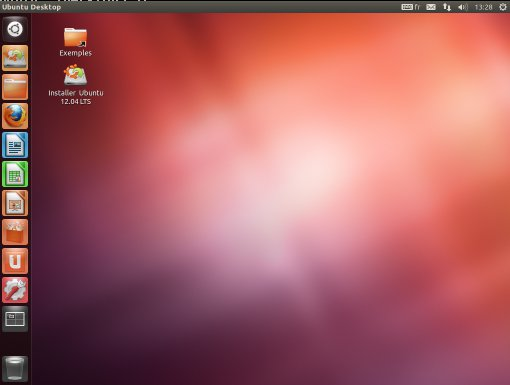
\includegraphics[height=3.5cm]{unity.jpg}
%
%\textit{Ubuntu}
%%\caption{Kbuntu}
%%\label{}
%%\label{essai1}
%\end{center}
%\end{minipage} \hfill
%\begin{minipage}[c]{.33\linewidth}
%\begin{center}
%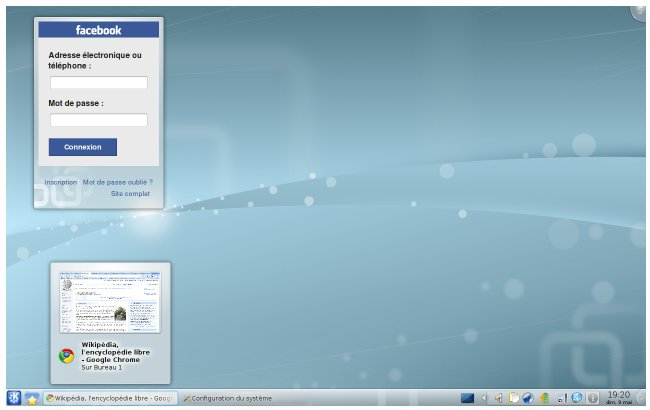
\includegraphics[height=3.5cm]{kbuntu.jpg}
%%\caption{Kubuntu, basé sur KDE}
%
%\textit{Kubuntu, basé sur KDE}
%%\label{}
%%\label{essai1}
%\end{center}
%\end{minipage} \hfill
%\begin{minipage}[c]{.33\linewidth}
%
%\begin{center}
%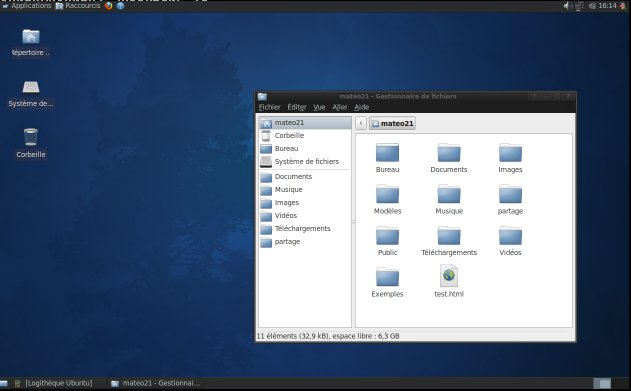
\includegraphics[height=3.5cm]{xbuntu.jpg}
%%\caption{Xubuntu, basé sur XFCE}
%
%\textit{Xubuntu, basé sur XFCE}
%%\label{}
%%\label{essai1}
%\end{center}
%\end{minipage} 
%\end{figure}
%
%\subsection{Identification des utilisateurs}
%
%Les systèmes d'exploitation Unix comme Microsoft sont multi-utilisateur : chaque utilisateur
%dispose d'un identifiant auprès du système (et en général, d’un mot de passe correspondant).
%
%\begin{figure}[h]
%\begin{minipage}[c]{.49\linewidth}
%\begin{center}
%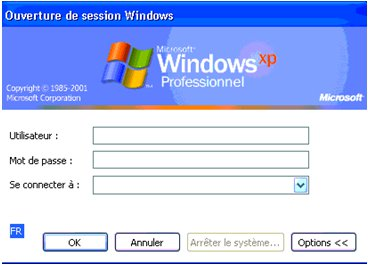
\includegraphics[height=5cm]{loginWin.jpg}
%
%\textit{Fenêtre d'identification de Windows}
%%\caption{Fenêtre d'identification de Windows}
%%\label{}
%\end{center}
%\end{minipage} \hfill
%\begin{minipage}[c]{.49\linewidth}
%\begin{center}
%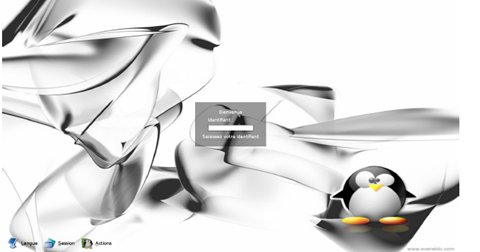
\includegraphics[height=5cm]{loginLin.jpg}
%
%\textit{Fenêtre d'identification de Linux}
%%\label{}
%\end{center}
%\end{minipage}
%\end{figure}
%
%%
%%Vous disposez d'un compte Windows avec des droits d'utilisateur limités accessible depuis n’'importe quel ordinateur du lycée sur le réseau Pédagogique.
%%\begin{itemize}
%%\item login: prénom.nom
%%\item mdp: date de naissance au format JJMMAAAA
%%\end{itemize}
%%
%%Vous pouvez dès à présent changer votre mot de passe pour sécuriser l’accès à votre compte.
%%
%%
%%Un compte utilisateur vous à été créé dans le système informatique, auquel est associé un identifiant,
%%et un mot de passe. 
%%De plus vous avez été déclaré comme
%%étant membre d'un ou plusieurs groupes d'utilisateurs, ce qui va vous donner certains droits
%%vis-à-vis du système informatique. 
%
%
%%
%%\subsection{Shell et interface graphique}
%%
%%Après avoir reconnu l'identifiant et le mot de passe comme valide le système
%%d'exploitation lance un programme (ou un ensemble de programmes)
%%qu'on appelle parfois shell. 
%%Il existe aussi des shells en mode texte, on les appelle alors aussi interprètes de commandes :
%%ce sont des programmes qui attendent une commande de l'utilisateur sous forme d'une
%%ligne de texte, l'exécutent, attendent de nouveau une commande, l'exécutent, etc. Ils étaient
%%historiquement utilisés sur des terminaux en mode texte, c'est-à-dire, une combinaison
%%d’un clavier et d’un écran incapable d'afficher autre chose que du texte en orange sur fond
%%noir (ou en vert sur fond noir). Aujourd'hui, ces terminaux ont quasiment disparu mais tous
%%les systèmes Unix proposent des émulateurs de terminaux.
%%
%%
%%\begin{figure}[h]
%%\begin{minipage}[c]{.49\linewidth}
%%
%%Un tel émulateur est présenté
%%ici. Les trois commandes pwd, ls et date on été tapé afin d'afficher le nom du répertoire de travail (print working directory), de lister son
%%contenu et d'afficher la date et l'heure. Il a ensuite tapé une commande plus compliquée,
%%qui permet en une ligne, certes complexe, de savoir combien de fichiers sont présents sur
%%l'ordinateur (on peut lire à la suite la réponse de la machine).
%%
%%\end{minipage} \hfill
%%\begin{minipage}[c]{.49\linewidth}
%%\begin{center}
%%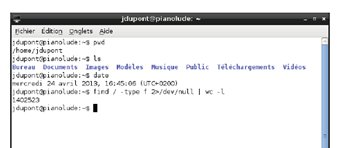
\includegraphics[width=.8\textwidth]{shell.jpg}
%%\caption{Exemple de shell}
%%\label{}
%%\label{essai1}
%%\end{center}
%%\end{minipage}
%%\end{figure}
%
%
%
%\subsection{La structure des dossiers et fichiers}
%
%Le nombre de fichiers étant généralement élevé, ils sont organisés en une structure arborescente
%de répertoires. Du point de vue de l'utilisateur, un répertoire est un ensemble de fichiers et de sous répertoires, désignés par des noms.
%%
%%\begin{savoir}
%%\textsc{SAVOIR-FAIRE Utiliser un système de fichiers}
%%
%%Dans un système de fichiers préexistant, il faut savoir :
%%\begin{itemize}
%%\item Se repérer dans l'arborescence. Cela demande de connaître dans les grandes
%%lignes la structure du système de fichiers, de savoir retrouver
%%son répertoire personnel et d'en connaître également l'organisation.
%%\item Se déplacer dans cette arborescence, au moyen des fenêtres d'un shell graphique
%%ou d'une commande (cd dans la plupart des systèmes d'exploitation). 
%%\end{itemize}
%%
%%\end{savoir}
%
%Du point de vue conceptuel, un fichier est une séquence finie d'octets, sans signification
%a priori : c'est le programme qui lira cette séquence d'octets qui décidera de la façon de
%la comprendre. Il peut contenir des données de tout type : texte, son, vidéo et même des
%programmes directement exécutables par le processeur (programmes dits « binaires » ou
%« en langage machine »).
%
%Les fichiers présents sur le disque dur sont répertoriés dans une ou plusieurs tables, stockées
%à un endroit du disque conventionnellement fixé, qui donnent des informations relatives
%à ces fichiers, appelées métadonnées, notamment :
%\begin{itemize}
%\item date de création, de dernière modification, de dernière lecture;
%\item taille du fichier;
%\item emplacement des données du fichier sur le disque;
%\item suivant les systèmes de fichiers employés, un numéro identifiant le fichier, appelé
%inode sous Unix.
%\end{itemize}
%
%La table des métadonnées est aussi appelée table des inodes. Du point de vue du système d'exploitation, un répertoire est juste un fichier particulier,
%qui contient une liste de couples $(n, i)$ où $n$ est un nom de fichier et $i$ l'inode du fichier.
%Une information supplémentaire est stockée dans la table des inodes pour indiquer, pour
%chaque fichier, s'il s'agit d'un fichier de données ordinaire ou d'un répertoire.
%
%
%\subsubsection{La racine}
%
%Dans un système de fichiers, il y a toujours ce qu'on appelle une racine, c'est-à-dire un gros dossier de base qui contient tous les autres dossiers et fichiers.
%
%Sous Windows, il y a en fait plusieurs racines. \textit{C:\textbackslash} est la racine de votre disque dur, \textit{D:\textbackslash} est la racine de votre lecteur CD (par exemple).
%
%Sous Linux, il n'y a qu'une et une seule racine : « / ». Il n'y a pas de lettre de lecteur car justement, Linux ne donne pas de nom aux lecteurs comme le fait Windows. Il dit juste « La base, c'est / ».
%
%Il n'y a pas de dossier de plus haut niveau que /, c'est-à-dire qu'il n'existe pas de dossier qui contienne le dossier /. Quand on est à la racine, on ne peut pas remonter en arrière car… on est déjà tout au début.
%
%\subsubsection{Architecture des dossiers}
%
%Sous Windows, un dossier peut être représenté de la manière suivante : \textit{C:\textbackslash Program Files\textbackslash Gimp 2}. On dit que Gimp 2 est un sous-dossier du dossier Program Files, lui-même situé à la racine.
%
%Vous noterez que c'est l'antislash \textbackslash (aussi appelé backslash) qui sert de séparateur aux noms de dossiers. Sous Linux, c'est au contraire le / (slash) qui sert de séparateur.
%Il n'y a pas de \textit{C:} sous Linux, la racine (le début) s'appelant juste /.
%
%Le dossier de notre superprogramme ressemblerait plutôt à quelque chose comme cela : \textit{/usr/bin/}. On dit que \textit{bin} est un sous-dossier du dossier \textit{usr}, lui-même situé à la racine.
%
%\begin{figure}[h]
%\begin{minipage}[c]{.49\linewidth}
%\begin{center}
%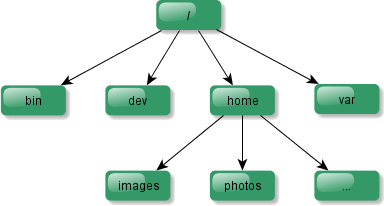
\includegraphics[width=.9\textwidth]{archilin.png}
%\textit{Organisation des dossiers de Linux}
%\end{center}
%\end{minipage} \hfill
%\begin{minipage}[c]{.49\linewidth}
%
%Sous Windows, on a l'habitude de trouver souvent les mêmes dossiers à la racine : Documents and Settings, Program Files, Windows… Sous Linux, vous vous en doutez, les dossiers sont complètement différents. 
%\newline\newline
%
%Quelques dossiers courants sous linux:
%\begin{itemize}
%\item \textit{boot} : fichiers permettant le démarrage de Linux;
%\item \textit{etc} : fichiers de configuration;
%\item \textit{home} : répertoires personnels des utilisateurs. On en a déjà parlé un peu avant : c'est dans ce dossier que vous placerez vos fichiers personnels, à la manière du dossier Mes documents de Windows.
%\end{itemize}
%\end{minipage}
%\end{figure}
%
%
%\subsubsection{Quelques commandes classiques pour se déplacer dans l'arborescence:}
%
%\begin{itemize}
%\item \textit{pwd} : afficher le dossier actuel
%\item \textit{ls} : lister les fichiers et dossiers
%\item \textit{cd}: changer de dossier
%\item \textit{du}: taille occupée par les dossiers
%\item \textit{cp} : copier un fichier
%\item \textit{mv} : déplacer un fichier
%\item \textit{rm} : supprimer des fichiers et dossiers
%\item \textit{mkdir} : créer un dossier
%\end{itemize}
%
%
%Ces quelques fonctions peuvent s'avérer nécessaires car elles sont utilisables dans Python pour manipuler les fichiers. 
%
%%Utiliser le joker *
%
%Le symbole * est appelé joker, ou encore wildcard en anglais sous Linux. 
%
%%\begin{minipage}[c]{.46\linewidth}
%%\begin{term}
%
%Le joker vous permet de copier par exemple tous les fichiers image .jpg dans un sous-dossier :
%%\begin{termi}[h]
%%cp *.jpg mondossier/
%%\end{termi}
%%\end{term}
%%\end{minipage}\hfill
%%\begin{minipage}[c]{.46\linewidth}
%%\begin{term}
%%Vous pouvez aussi vous en servir pour copier tous les fichiers dont le nom commence par « so » :
%%\begin{termi}[h]
%%cp so* mondossier/
%%\end{termi}
%%\end{term}
%%\end{minipage}
%
%\subsection{Droits d’accès}
%
%Les droits d'accès font partie des propriétés d'un fichier. On peut recenser 3 principaux droits pour un fichier : 
%\begin{itemize}
%\item le droit en lecture (\textit{r -- read}), qui permet à l'utilisateur de lire le contenu du fichier;
%\item le droit en écriture (\textit{w -- write}), qui permet à l'utilisateur d'écrire dans le fichier;
%\item le droit d'exécution (\textit{x -- execute}), qui permet à l'utilisateur d'exécuter le fichier.
%\end{itemize}
%
%Par ailleurs pour un même ordinateur, il peut exister plusieurs utilisateurs. Ces utilisateurs peuvent de plus appartenir à un groupe.
%
%Ainsi il est possible de distribuer des droits à un utilisateur, à un groupe d'utilisateurs ou à tous les utilisateurs.  
%
%\begin{minipage}[c]{.45\linewidth}
%\begin{center}
%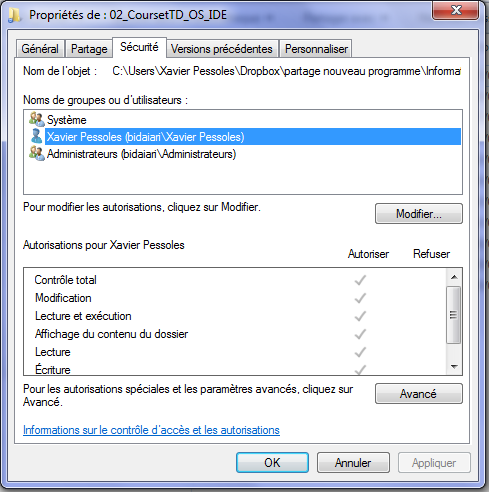
\includegraphics[width=.85\textwidth]{droits_win.png}
%\end{center}
%\end{minipage}\hfill
%\begin{minipage}[c]{.45\linewidth}
%\begin{center}
%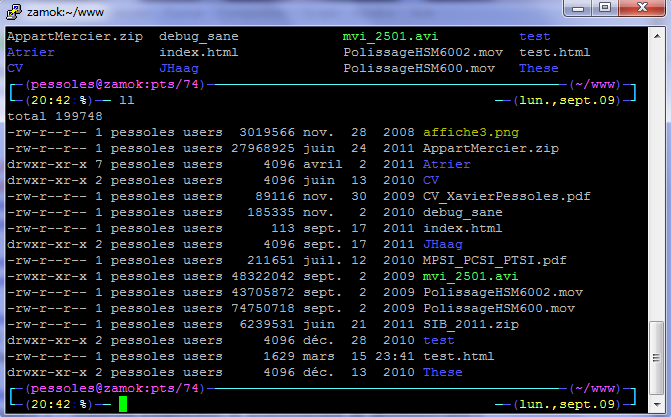
\includegraphics[width=.8\textwidth]{droits_lin.png}
%$$
%-\underbrace{rw-}_{1}\underbrace{r--}_{2}\underbrace{r--}_{3}
%$$
%\begin{itemize}
%\item 1 : droits pour l'utilisateur pessoles;
%\item 2 : droits pour l'utilisateur user;
%\item 3 : droits pour le reste du monde.
%\end{itemize}
%\end{center}
%\end{minipage}
%
%%Vous êtes inscrit dans un groupe associé à la classe dans laquelle vous êtes. Vous avez accès en lecture/écriture dans Poste de travail/groupes au répertoires d'échanges de la classe. C'est données son stockées sur un serveur distant est accessible sur tous les ordinateur du lycée.
%
%\begin{warn}
%Toutes les données que ce soit dans votre espace personnel ou sur les serveurs du lycée ne sont stockées qu'a titre provisoire. Il vous appartient de faire des sauvegardes régulières.
%\end{warn}
%
%
%\begin{warn}
%Tenter d'accéder aux données d'autrui est considéré comme une atteinte à la vie privée.
%\end{warn}
%
%%Chaque entrée de la table des inodes comporte, en plus des métadonnées déjà mentionnées,
%%les droits d'accès accordés aux utilisateurs du système. Ces droits, appelés aussi permissions,
%%précisent qui a le droit de faire quoi sur le fichier ou le répertoire concerné (lecture/écriture/exécution). Pour
%%voir ces permissions, il suffit d'effectuer un clic droit dans le gestionnaire de fichiers sur
%%le répertoire, de choisir « Propriétés » dans le menu contextuel qui apparaît alors, puis de
%%cliquer sur l’onglet « Permissions ». 
%
%
%%\subsection{Lancement d'applications}
%%
%%\begin{savoir}
%%\textsc{SAVOIR-FAIRE Lancer des applications}
%%
%%Pour lancer une application (un programme), on dispose essentiellement de deux
%%possibilités :
%%\begin{itemize}
%%\item Cliquer sur un bouton, un menu ou un fichier du shell graphique. Cette méthode
%%est en général à réserver pour des tâches simples ; elle offre l’avantage d’être
%%intuitive et donc utilisable même par des utilisateurs débutants.
%%\item Taper une commande dans un shell en mode texte. Dès que l'on veut exprimer des
%%commandes plus complexes, comme par exemple passer des arguments à un
%%programme ou manipuler des fichiers en masse, cette méthode s'avère quasi
%%incontournable. Son utilisation est plus ou moins facilitée selon le système
%%d'exploitation que l'on utilise.
%%\end{itemize}
%%
%%Une fois que le système a constaté que l'utilisateur avait le droit d'exécution sur le programme,
%%il réserve un espace dans la mémoire vive de l'ordinateur pour stocker les instructions
%%du programme ainsi que ses données. Il copie le contenu du fichier exécutable en
%%mémoire.
%%Celui-ci n'est qu'une suite de bits qui codent les instructions dans le langage du processeur
%%(on dit que le programme est en langage machine), il peut donc les exécuter en effectuant
%%un branchement vers les premières instructions du programme.
%%
%%Lorsqu'on clique sur le nom ou l'icône d'un fichier, le gestionnaire de fichiers commence
%%par déterminer de quel type de fichier il s'agit. Suivant les systèmes, il peut s'appuyer sur
%%diverses informations :
%%\begin{itemize}
%%\item Le nom du fichier et tout particulièrement son suffixe. Ainsi un fichier dont le nom se
%%termine par .odt sera t-il identifié comme un fichier OpenDocument (le gestionnaire
%%consulte pour cela une table qui associe un type de fichier à chaque suffixe connu).
%%\item Le contenu du fichier.
%%\item Le fait que l'utilisateur ait ou non le droit d’exécuter ce fichier.
%%\item Sur certains systèmes (Mac OS X en particulier) : métadonnées associées au fichier
%%donnant son type.
%%\end{itemize}
%%Puis, une fois le type déterminé, il consulte une table (commune à tout le système ou
%%spécifique au gestionnaire de fichiers, commune à tous les utilisateurs ou spécifique à l'utilisateur)
%%indiquant à quelle application est associé ce type de fichier. Il lance alors l'application,
%%en lui fournissant pour argument (c'est-à-dire comme information supplémentaire)
%%le nom du fichier à ouvrir. Là encore, la situation est exactement la même que si on avait
%%tapé ooffice nomdufichier dans un shell en mode texte.
%%\end{savoir}
%%
%%
%%\begin{savoir}
%%\textsc{SAVOIR-FAIRE Écrire un programme et le lancer}
%%
%%Tout utilisateur peut écrire ses propres programmes. Il existe pour cela essentiellement
%%trois possibilités :
%%\begin{itemize}
%%\item Les écrire en langage machine. C'est une tâche ardue car le langage machine est un
%%langage de bas niveau dans lequel il est difficile ou au minimum fastidieux
%%d'implanter des idées un tant soit peu complexes.
%%\item Utiliser un compilateur. Il s'agit d'un outil traduisant un programme écrit dans un
%%langage évolué en un programme en langage machine. Plus précisément, dans
%%le cas du langage C par exemple, on pourra ainsi, à partir d'un fichier contenant
%%le texte d'un programme C (appelé par exemple hello.c), produire un
%%programme en langage machine (appelé par exemple hello).
%%\item Faire appel à un interpréteur d'un langage évolué. Un interpréteur est un programme
%%exécutable qui va lire le texte d'un programme dans un langage évolué
%%pour l'exécuter pas à pas, sans passer par la phase intermédiaire de compilation.
%%La compilation demande donc un traitement préliminaire avant de pouvoir exécuter le
%%programme que l'on a écrit, mais produit en général des applications efficaces. À l'inverse,
%%on peut interpréter un programme immédiatement après l'avoir écrit, mais il aura tendance
%%à s'exécuter moins rapidement. \textbf{C'est vers cette solution que l'on va s'orienter au départ.}
%%
%%\end{itemize}
%%
%%Le choix entre compilation et interprétation dépend très largement du langage dans lequel
%%on programme : certains ne proposent qu'une seule des deux possibilités, d'autres laissent
%%le choix. Il existe même des situations intermédiaires où un programme peut être compilé
%%dans un langage qui est plus proche du langage machine mais qui doit encore être interprété
%%(on parle de bytecode).
%%\end{savoir}
%
%
%\section{Python}
%
%
%\begin{minipage}[c]{.79\linewidth}
%
%Python est un langage de programmation, dont la première version est sortie en 1991. Créé par Guido van Rossum, il a voyagé du Macintosh de son créateur, qui travaillait à cette époque au Centrum voor Wiskunde en Informatica aux Pays-Bas, jusqu'à se voir associer une organisation à but non lucratif particulièrement dévouée, la Python Software Foundation, créée en 2001. Ce langage a été baptisé ainsi en hommage à la troupe de comiques les « Monty Python ».
%
%\subsection{À quoi peut servir Python ?}
%\end{minipage} \hfill
%\begin{minipage}[c]{.2\linewidth}
%\begin{center}
%\includegraphics[width=.99\textwidth]{monty.jpg}
%%\label{}
%\end{center}
%\end{minipage}
%
%
%
%
%Python est un langage puissant, relativement facile à apprendre et riche en possibilités. Il est possible d'étendre ses fonctionnalités. On peut aussi appeler des bibliothèques qui aident le développeur à travailler. 
%
%%Dès l'instant où vous l'installez sur votre ordinateur, vous disposez de nombreuses fonctionnalités intégrées au langage que nous allons découvrir tout au long de ce livre.
%%Il est, en outre, très facile d'étendre les fonctionnalités existantes, comme nous allons le voir. Ainsi, il existe ce qu'on appelle des bibliothèques qui aident le développeur à travailler sur des projets particuliers. Plusieurs bibliothèques peuvent ainsi être installées pour, par exemple, développer des interfaces graphiques en Python.
%
%Python permet :
%\begin{itemize}
%\item de réaliser de petits programmes très simples, appelés scripts, chargés d'une mission très précise sur votre ordinateur;
%\item des programmes complets, comme des jeux, des suites bureautiques, des logiciels multimédias, des clients de messagerie…
%\item des projets très complexes, comme des progiciels (ensemble de plusieurs logiciels pouvant fonctionner ensemble, principalement utilisés dans le monde professionnel).
%\end{itemize}
%
%Voici quelques-unes des fonctionnalités offertes par Python et ses bibliothèques :
%\begin{itemize}
%\item créer des interfaces graphiques ;
%\item faire circuler des informations au travers d'un réseau ;
%\item dialoguer d'une façon avancée avec votre système d'exploitation ;
%\item ...
%\end{itemize}
%
%\subsection{ Un langage de programmation interprété}
%Python est un langage de programmation interprété, c'est-à-dire comme on l'a spécifié au que les instructions que vous lui envoyez sont « transcrites » en langage machine au fur et à mesure de leur lecture. D'autres langages (comme le C / C++) sont appelés « langages compilés » car, avant de pouvoir les exécuter, un logiciel spécialisé se charge de transformer le code du programme en langage machine. On appelle cette étape la « compilation ». À chaque modification du code, il faut rappeler une étape de compilation.
%
%Les avantages d'un langage interprété sont la simplicité (on ne passe pas par une étape de compilation avant d'exécuter son programme) et la portabilité (un langage tel que Python est censé fonctionner aussi bien sous Windows que sous Linux ou Mac OS, et on ne devrait avoir à effectuer aucun changement dans le code pour le passer d'un système à l'autre). Cela ne veut pas dire que les langages compilés ne sont pas portables, loin de là ! Mais on doit utiliser des compilateurs différents et, d'un système à l'autre, certaines instructions ne sont pas compatibles, voire se comportent différemment.
%
%En contrepartie, un langage compilé se révélera bien plus rapide qu'un langage interprété (la traduction à la volée de votre programme ralentit l'exécution), bien que cette différence tende à se faire de moins en moins sentir au fil des améliorations. De plus, il faudra installer Python sur le système d'exploitation que vous utilisez pour que l'ordinateur puisse comprendre votre code.
%
%\subsection{Différentes versions de Python}
%
%Lors de la création de la Python Software Foundation, en 2001, et durant les années qui ont suivi, le langage Python est passé par une suite de versions que l'on a englobées dans l'appellation Python 2.x (2.3, 2.5, 2.6…). Depuis le 13 février 2009, la version 3.0.1 est disponible. Cette version casse la compatibilité ascendante qui prévalait lors des dernières versions.
%
%%Installation à la maison : https://code.google.com/p/pythonxy/wiki/Downloads?tm=2
%
%
%
%
%
%
%\begin{thebibliography}{2}
%\bibitem{Tous}{Wack, Conchon, Courant, deFalco, Dowek, Filliatre, Gonnord, Informatique pour tous en classes préparatoires aux grandes écoles, éditions Eyrolles.}
%\bibitem{zero}{Apprenez à programmer en Python \url{http://www.siteduzero.com/}.}
%\end{thebibliography}
%
%\footnotesize
%
%\begin{thebibliography}{2}
%\bibitem{medevielle}{François Médevielle, Architecture des ordinateurs -- UPSTI}
%\bibitem{beynet}{Patrick Beynet, ISN -- Architectures matérielles -- Architecture des ordinateurs. Lycée Rouvière.}
%
%\bibitem{wikipedia}{\url{http://fr.wikipedia.org/wiki/Disque_dur}.}
%\bibitem{ccm}{\url{http://www.commentcamarche.net/contents/740-disque-dur}.}
%
%\bibitem{cm}{Carte mère. \url{http://micropuces-informatique.fr/?page_id=29}}
%\bibitem{ram}{\url{http://nouvelleteckno.files.wordpress.com/2011/11/ddr.jpg}}
%\bibitem{dd1}{\url{http://www.builttoordercomputers.com/wp-content/uploads/2011/04/Hard-Disk-Drive-1.jpg}}
%\bibitem{dd2}{\url{http://www.reviversoft.com/blog/wp-content/uploads/2013/01/hard_drive_problems_harddrive_02.jpg}}
%\bibitem{dd_ssd}{\url{http://www.militarysystems-tech.com/files/militarysystems/imagecache/Original/supplier_images/Solid\%20State\%20Drive\%20SSD\%20Galatea\%20100GB\%20200GB\%20Encryption-l.jpg}}
%\bibitem{usb}{\url{http://fr.ids-imaging.com/store/media/catalog/product/cache/4/image/795x795/9df78eab33525d08d6e5fb8d27136e95/u/s/usb2_cable_standard_2.jpg}}
%\bibitem{ps2}{\url{http://www.baybits.eu/174-607-thickbox/adaptateur-convertisseur-usb-ps2-ps-2-clavier-et-souris.jpg}}
%\bibitem{ethernet}{\url{http://brain.pan.e-merchant.com/2/4/46000142/l_46000142.jpg}}
%\bibitem{cm2}{Carte mère. \url{http://serveurfelix.myds.me/~Felix/HTTrack/doku505c.html?id=architecture_pc:architecture_pc:composants}}
%\bibitem{usb}{\url{http://u.s.b.free.fr/pdf/L_USB_et_sa_norme_v1.pdf}}
%\end{thebibliography}
